\documentclass{homework}

\title{RAMLAB Internship \\ Progress Report}
\author{Ulf Torsten Kemmsies - 4794281  \\
MSc. Space Engineering - TU Delft}
\usepackage{geometry}
\usepackage{graphicx}
\graphicspath{ {./images/} }
\usepackage{amsmath}
\usepackage[table,xcdraw]{xcolor}
\usepackage{lscape}
\usepackage{multicol} % For multiple columns
\usepackage{capt-of} % For creating captions outside of floats
\usepackage{float}

\begin{document}

\maketitle

\begin{abstract}

\end{abstract}

\begin{center}
Github repository: \url{test}
\end{center}

\begin{multicols}{2} % Start two-column layout


% \begin{minipage}{\linewidth}
%       \centering
%       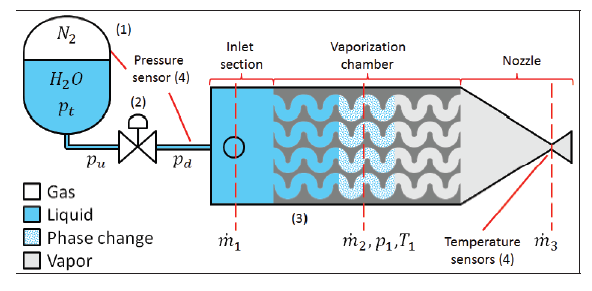
\includegraphics[width=\linewidth]{images/overview.png}
%       \captionof{figure}{Picture example}
%       \label{fig:model_overview}
%   \end{minipage}

% Add literature review section

\section*{Introduction}

This report is a recollection of the internship done, as required by the
Delft University of Technology, in pursuit of the MSc. in Space Engineering,
by the author at, the Rotterdam
Additive Manufacturing Laboratory, more commonly known as RAMLAB.

This internship, broadly speaking, was an investigation into the
application of Wire Arc Additive Manufacturing (WAAM) to the production of
metallic parts with magnetic properties.

WAAM is a production process used to 3D print or repair metal parts. It belongs to the Direct Energy Deposition (DED) family of Additive Manufacturing processes. The process is executed by depositing layers of metal on top of each other until a desired 3D shape is created. This is achieved by a welding robot integrated with a power source.

The report will start with a brief introduction to the company, followed by
a description of the problem that was investigated. The methods used to
investigate the problem will be described, followed by the outcome of the
investigation. The report will conclude with a summary of the conclusions
drawn from the investigation, and recommendations for future work.


\section{Company Background}

RAMLAB, based in Rotterdam, is a pioneer in the field of 3D metal printing, monitoring, and analysis solutions for Wire Arc Additive Manufacturing (WAAM). They are known for their high-quality WAAM systems and have developed MaxQ, a quality monitoring and control system for WAAM.

RAMLAB has three founding partners: Port of Rotterdam, InnovationQuarter and RDM Next, and collaborates with many other partners from academia, industry and government. RAMLAB conducts several research projects on WAAM, such as WAAMTOP, Grade2XL, AiM2XL and SMITZH.

RAMLAB's WAAM technology offers several advantages over conventional manufacturing processes. It allows for the manufacturing of large parts with dimensions over a cubic meter, offers additional design freedom, and uses a wide range of materials. It also offers the possibility of designing functionally graded components, where multiple materials can be combined to design a part.

They made headlines in 2017 by 3D printing a full-scale prototype of the world's first class approved ship's propeller. Their work continues to push the boundaries of what's possible in additive manufacturing - currently, they are working on manufacturing several-meter-wide pressure vessels for underwater structures, an unprecended feat in the field of additive manufacturing.




\section{Problem Introduction}

The project, which is aimed at investigating the potential of 3D metallic printing using WAAM, is focused on an Iron-Cobalt (Fe-Co) alloy called Vacoflux-17 known for its superior magnetic properties.

Vacoflux 17 is a type of Fe-Co alloy that has excellent magnetic properties and can be used for high performance magnetic actuators. It is produced by VACUUMSCHMELZE GmbH \& Co. KG, a company that specializes in advanced magnetic solutions.
Vacoflux 17 can be supplied in various forms, such as strip material, stamped parts, solid rods, and wire material. It has a saturation polarization of 2.22 T, an electrical resistivity of 0.41 $\mu \Omega m$, and a Curie temperature of 920 °C.

It can be heat treated in hydrogen atmosphere to improve its mechanical properties and reduce its iron losses. Vacoflux 17 is suitable for applications such as components and actuators for the automotive industry, especially diesel injection, and rotors and stators of electrical motors and generators.

The overarching goal of the investigation is to manufacture simple multilayer geometries that retain the material's base mechanical and magnetic properties with a minimum finish quality and geometric accuracy.

Inititally in the internship, the processability of the Fe-Co alloy is to be evaluated and its microstructural evolution during deposition using WAAM is to be understood. This involves conducting a series of experiments to observe the alloy's behavior under various conditions and analyzing the resulting depositions. The objective is to acquire a comprehensive understanding of how the alloy reacts to the WAAM process and how its properties are altered by deposition.

The focus then transitions towards developing deposition procedures that enable successful 3D printing of the Fe-Co alloy. This involves further experimentation and analysis, with an emphasis on optimizing process parameters to achieve desired material properties. The final part of this stage involves characterizing the material properties of the printed Fe-Co alloy, including its magnetic properties.

Throughout both stages, supervision is provided by experts from RAMLAB and TU Delft. Training in relevant techniques and methodologies is received, a thorough literature review is conducted, experiments are carried out, and results are analyzed. This project offered a unique opportunity to gain hands-on experience in 3D metallic printing and contribute to cutting-edge research in this field.

\section{Literature Review and Background Information}

\subsection{MIG WAAM}

(Metal Inert Gas) MIG WAAM consists depositing molten wire onto a workpiece using an electric arc between the wire and workpiece as a heat source. MIG welding uses inert gases for shielding and is suitable for non-ferrous metals like aluminum, while MAG (Metal Active Gas) welding uses active gas mixtures and is used for welding steel.

MIG and MAG differ from the other two main welding methods: TIG (Tungsten Inert Gas) welding uses an open arc shielded by inert gases like argon or helium, while PAW (Plasma Arc Welding) uses a constricted arc with the electrode positioned within the torch body, separating the plasma arc from the shielding gas envelope.

The main phases of MIG deposition are as follows:

\begin{enumerate}
    \item Arc Generation: The process begins with the generation of an electric arc between the wire electrode and the workpiece. This arc is hot enough to melt the wire electrode and part of the workpiece.
    \item Melting and Deposition: The melted wire, now in a liquid state, is then deposited onto the workpiece in a selective layered fashion.
    \item Solidification: Upon the solidification of the molten metal layer over a cold substrate, the subsequent thermal contraction of the metal layer generates tensile and compressive stresses respectively on the deposited layer and substrate.
    \item Heat Transfer and Fluid Flow: The heat transfer and fluid flow during this process play a crucial role in determining the final microstructure and mechanical properties of the deposited material.
\end{enumerate}

\subsubsection{Process parameters}

The main process parameters in MIG are current/wire feed rate, voltage, and travel speed, and wire feed rate, affect the bead geometry, mechanical properties, and deposition rate of the produced parts.


\textbf{Voltage} in welding primarily affects the width of the weld bead and the amount of spatter. Higher voltage settings result in a wider weld bead and more spatter.

The \textbf{welding current} affects the heat available to melt the welding wire and the base material. It is directly correlated to wire \textbf{feed rate}: when feed rate increases, so does the welding amperage. Higher amperage settings yield greater joint penetration.

\textbf{Travel speed} in welding primarily affects the size of the weld bead and heat input. An increase in travel speed leads to a decrease in heat input, resulting in a narrower weld bead and a smaller heat-affected zone. However, increasing the travel speed beyond a certain limit can lead to insufficient fusion and porosity in the weld. Conversely, slow travel speeds can cause excessive weld deposition, which commonly causes cold lapping or a lack of fusion.



\subsubsection{Cold Metal Transfer (CMT)}

CMT, or Cold Metal Transfer, is a welding process developed by Fronius that stands out due to its extremely low heat input and an significantly stable arc. The method boasts less distortion, 50\% less dilution of filler and base material, and higher welding speeds.
The digital process control detects a short circuit (wire touching workpiece) and then detaches the droplet by retracting the wire. During welding, the wire moves forward and is pulled back again as soon as the short circuit occurs, as shown in \autoref{fig:CMT}. Several different waveforms for this process have been developed, often catering to the different needs of specific materials, like NiCr, steel, and Al.
As a result, the arc only introduces any heat for a very brief period during the arc-burning phase. The short circuit is controlled and the current is kept low, resulting in a nearly spatter-free material transfer. The arc length is detected and adjusted mechanically. The arc remains stable, no matter what the surface of the workpiece is like or how fast the user welds.

\begin{minipage}{\linewidth}
    \centering
    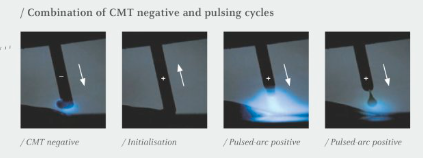
\includegraphics[width=\linewidth]{images/CMT_illustration.PNG}
    \captionof{figure}{CMT cycle}
    \label{fig:CMT}
\end{minipage}


\subsection{Soft Magnetic Materials}

Soft magnetic materials are materials that are easy to be magnetized and demagnetized, whereas hard magnetic materials keep their magnetization and are often permanent magnets.

\subsubsection{Magnetic property definitions}

\textbf{Saturation magnetization} occurs when an increase in the applied magnetic field no longer increases the magnetization of a material. This is due to the alignment of magnetic domains reaching their maximum, resulting in a leveling off of the total magnetic flux density.

\textbf{Magnetic coercivity}, also known as coercive force, is a measure of a ferromagnetic material's ability to resist demagnetization from an external magnetic field. It is measured in oersted or ampere/meter units. There are different types of coercivity, including normal coercivity, intrinsic coercivity, and remanence coercivity, each representing different aspects of demagnetization.

\textbf{Magnetic permeability}, denoted by the Greek letter \(\mu\), measures how a material reacts to a magnetic field. It is the ratio of the magnetic flux density established within the material to the magnetic field strength of the magnetizing field. In simpler terms, it indicates a material's ability to support the development of a magnetic field and its resistance to that field.

\textbf{Magnetic power losses}, also known as iron losses, occur in the core of magnetic components like transformers and inductors. These losses are caused by hysteresis and eddy currents. Hysteresis loss happens when a magnetic material lags behind changes in the magnetic field, dissipating energy as heat. Eddy current loss occurs due to induced currents in the core, producing heat. These losses impact the efficiency of electromagnetic devices, making their reduction crucial in device design.

The \textbf{Curie temperature} is the temperature at which materials lose their permanent magnetic properties and can be replaced by induced magnetism. At the Curie temperature, a material's intrinsic magnetic moments change direction, causing a transition from ordered to disordered magnetic moments.

\subsubsection{Properties of SMMs}

Soft magnetic materials possess several desirable properties that make them suitable for various applications.

High saturation magnetization: being able to store a significant amount of magnetic energy, makes them efficient for applications such as transformers, inductors, and magnetic storage devices. This property allows them to generate strong magnetic fields when exposed to an external magnetic field.

Low coercivity: they can easily switch their magnetization direction when subjected to an external magnetic field. This property is crucial for applications that require rapid magnetization and demagnetization cycles, such as in transformers and electric motors. Low coercivity ensures efficient energy conversion and reduces energy losses.

High initial/maximum permeability ($\mu_{max}$): they can quickly respond to changes in the magnetic field, allowing for efficient magnetic flux induction. This property is essential for applications like electromagnetic shielding, where the material needs to redirect magnetic fields away from sensitive components.

Low power losses.

High Curie temperature: they can magnetic properties at elevated temperatures. This property is desirable for applications that involve high-temperature environments, such as power electronics, where the material needs to retain its magnetic characteristics even under thermal stress.

\subsubsection{Fe-Co alloys}

Fe-Co alloys, depending on the manufacturing method, can be either amorphous or nanocrystalline. Amorphous and nanocrystalline soft magnetic materials have superior magnetic properties and durability compared to normal soft magnetic alloys. They exhibit lower coercivity, higher permeability, and lower eddy current losses, making them more efficient for power electronics and electrical machines.

Fe-Co alloys can have both the alpha and gamma phases, with the alpha phase being a solid solution based on the body-centered cubic structure and the alpha' phase being an ordered intermetallic phase formed by the primary crystallization of the amorphous alloy. The alpha' phase contributes to the excellent soft magnetic properties of the alloy.

\subsubsection{Microstructure and magnetic properties}

The microstructure of a material has a significant impact on its magnetic properties. Several key factors should be taken into account:

\textbf{Grain structure}: The arrangement of grains in the material can greatly influence its magnetic behavior. Different types of grain structures, such as planar, cellular, columnar dendritic, and equiaxed dendritic, can result in varying magnetic properties.

\textbf{Grain size}: The size of the grains also plays a role. For example, in FePt storage films used in heat-assisted magnetic recording media, the grains need to be smaller than 6 nm to achieve a specific areal density.

\textbf{Phase composition}: The composition of different phases within the material can affect its magnetic properties. In some cases, a microstructure with uniformly dispersed nanocrystals of specific compositions has been found to optimize magnetic properties.

% \textbf{Processing conditions}: The conditions under which the material is processed can impact its microstructure and, consequently, its magnetic properties.

\textbf{Microstructural features}: Certain features within the microstructure can enhance or diminish magnetic properties. For instance, complex microstructures tend to have higher coercivity and lower remanence than simple ones.

\subsection{Characterization techniques}

\subsubsection{Weld Characterization}



\subsubsection{Magnetic Characterization}

\subsection{Post treatment techniques}

\subsection{Previous work}





\section{Methods}

\subsection{Experimental Setup}

All tests were conducted at RAMLAB's facilities at the port of Rotterdam's Innovation Dock. The robotic printer, as shown in \autoref{fig:robot_setup}, is their customized Techman XXX 6-axis robot with a Fronius TPS 320i CMT-capable MIG power source.
Atop the welding torch mount sits a RAMLAB-developed MaxQ system, capable of performing 3D scans of the workpiece to determine geometric printing accuracy, as well as thermal scans to determine the interpass temperature between layers. Some tests were performed before the thermal camera was calibrated, and thus a simple two-wire thermocouple was used.
Additionally, a Cavitar camera was used to record later tests to inspect the solidification process.

\begin{minipage}{\linewidth}
      \centering
      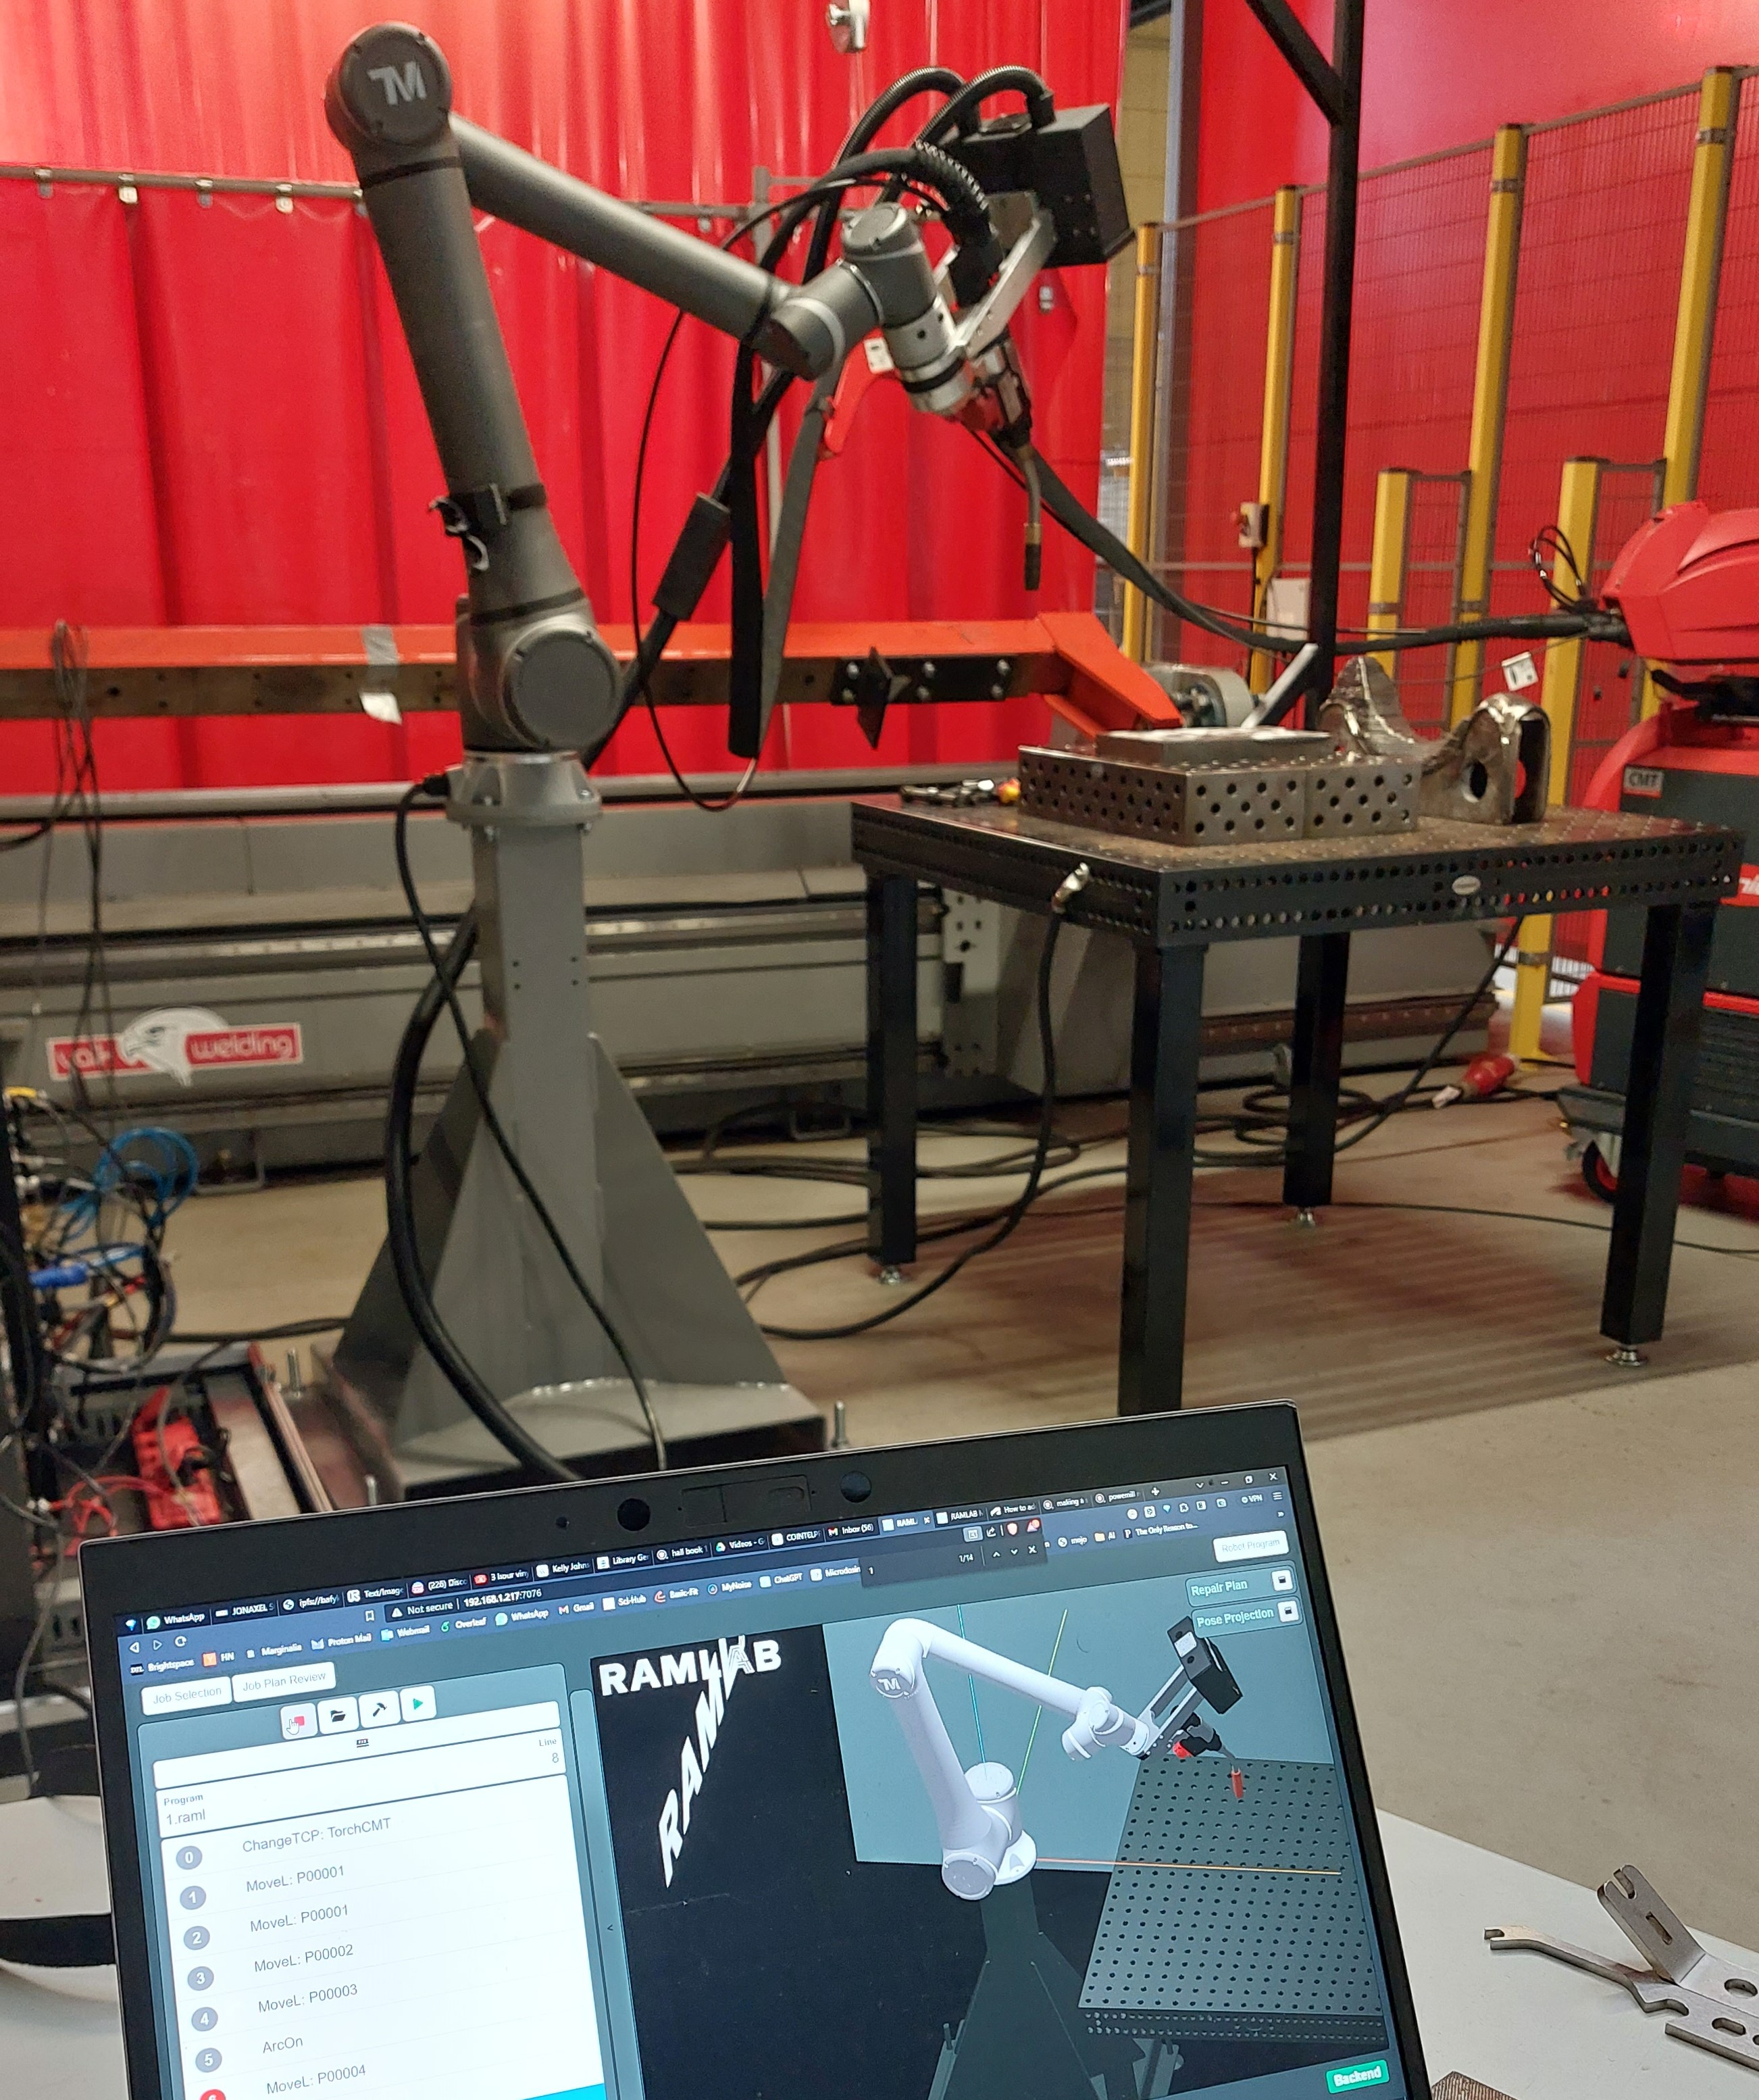
\includegraphics[width=\linewidth]{images/robot_setup.jpg}
      \captionof{figure}{Techman robot setup}
      \label{fig:robot_setup}
  \end{minipage}

The welds and geometries were created using Autodesk PowerShape and PowerMill and exported with RAMLAB's custom postprocessing software to make use of their MaxQ system.

The baseplates used were made of stainless steel with dimensions of 200x300x30 mm.

Because the Fronius power source does not yet have an experimental welder for the Fe-Co alloy, a welder program for a similar material was chosen. NiCrMo-3 has comparable atomic sizes to FeCo and also contains trace Molybdenum like Vacoflux 17, so it available welder program was chosen as a starting point. Because the Vacoflux 17 wire provided was 1 mm in diameter, the cladding (surface coating) preset was used, since it is optimized for lower deposition rates.

The shielding gas used was Alumaxx Plus X30S, composed of 30\% Helium and 70\% Argon, although the gas program used in the Fronius system was for pure Argon. The inclusion of Helium is important because of its high thermal conductivity, which disperses the arc energy, produces a wider and smoother arc, and allows for lower heat inputs and higher travel speeds. Combined with the use of CMT, this allows one to weld in significantly colder conditions than usual.

\subsection{Experimental Procedure}

The main objectives of this material characterization can be categorized as the following milestones:

\begin{enumerate}
    \item Minimum weldability for single beads
    \item Minimum weld quality for single beads and overlapping beads
    \item Minimum weld quality for single bead layers
    \item Process stability over many single-bead layers
    \item Minimum print quality for a full-scale part
    \item Magnetic and material property maintenance of samples and final part
\end{enumerate}

Instead of planning out all the experiments beforehand, the project was conducted in an iterative fashion, with each experiment informing the next. This was done to make the most of the limited time available and to ensure that the project would be able to reach the final milestone in the time available.

The process parameters were iteratively changed between welds, albeit with some limitations. The Fronius power source has feed rate/current/voltage relationships (called "welders") that have been experimentally determined for several materials, and these cannot be changed freely nor allow for independent control over the parameters. Because of this, only the feed rate was controlled for.

The process parameters that were altered for all welds were the following: feed rate, travel speed, SFI (Spatter Free Injection), arc length correction, initial current level (as a percentage of the main current) and initial current slope time.

The Spatter Free Injection by Fronius, also known as the Low Spatter Control (LSC) process, is a modified dip transfer arc welding process that achieves high-quality weld seams with minimal spattering and an increased deposition rate by triggering the short circuit at a low current level, leading to a gentle reignition and a stable welding process.

The arc length correction is a percentual correction of the distance between the tip of the wire and the workpiece, and since this distance is small, even small percentual changes can have an outsized effect. The initial current level is the percentage of the main current that is used for the initial arc ignition, and the initial current slope time is the time it takes for the current to ramp up to the main current level.

For overlapping beads, the spacing between beads was controlled. For layered single-bead walls, the layer height was taken as the running average of the wall, and the interpass temperature was controlled.




% \section{Results}

\begin{minipage}{\linewidth}
    \centering
    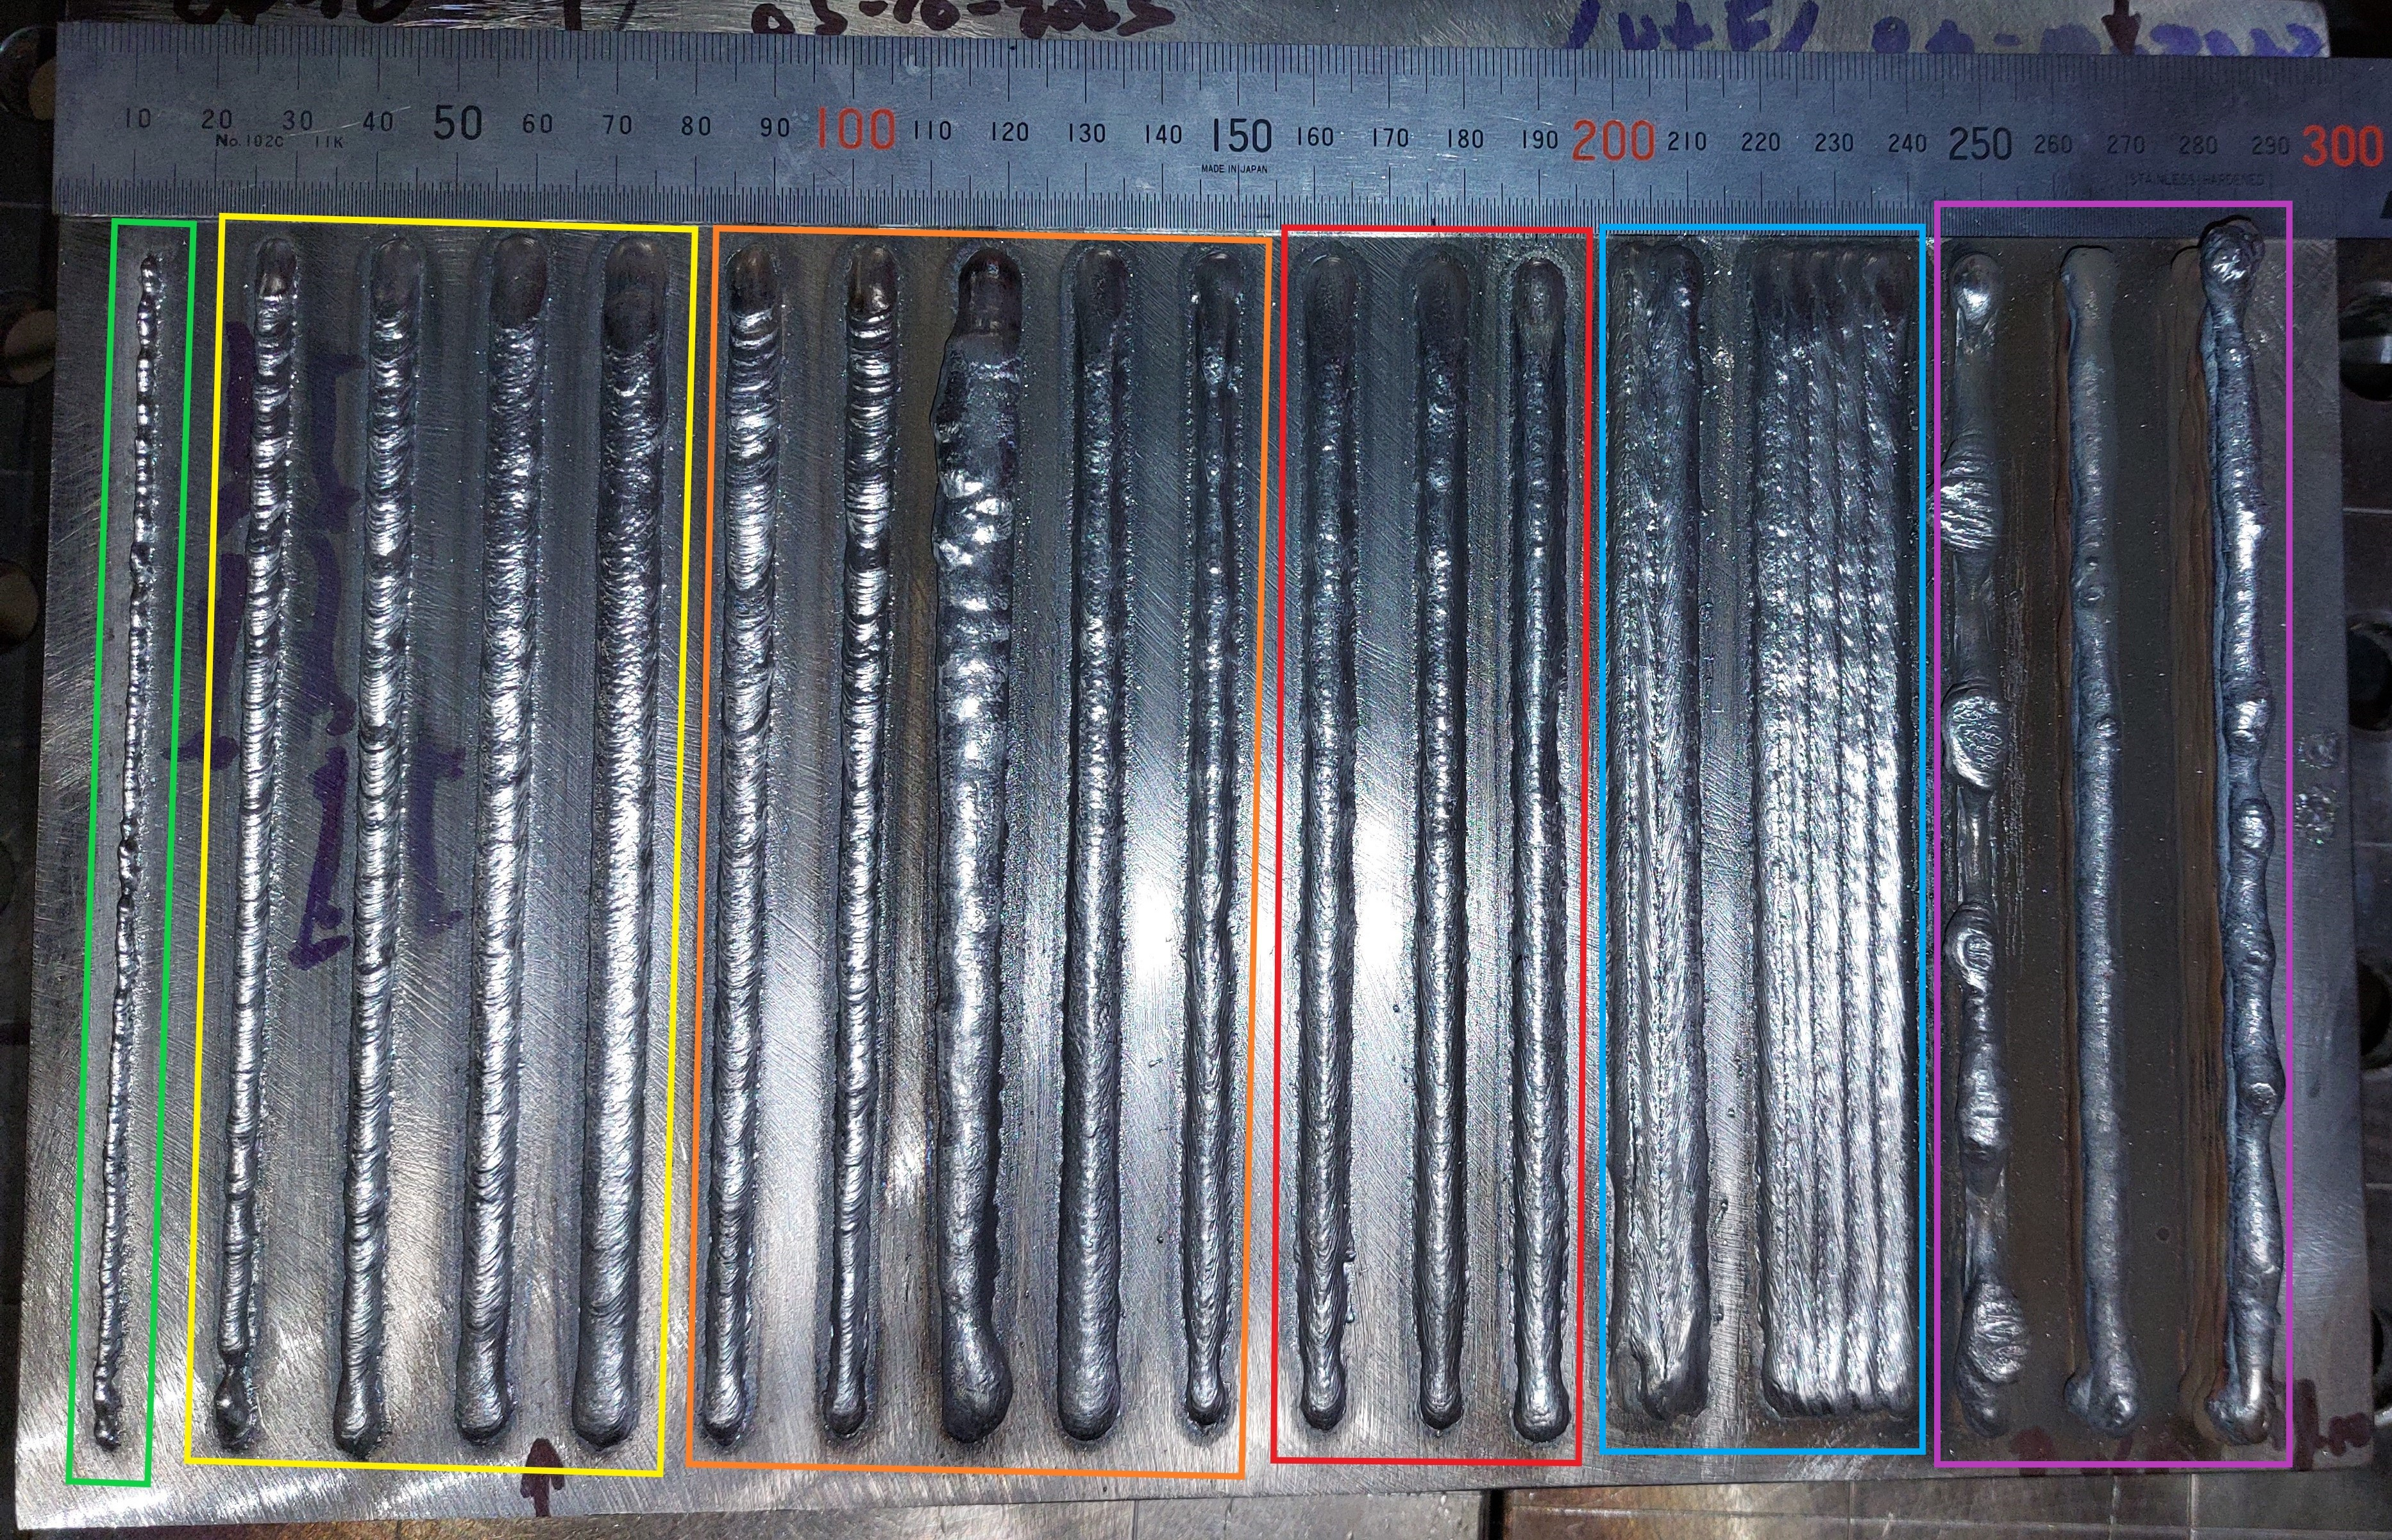
\includegraphics[width=\linewidth]{images/all_welds_boxes.jpg}
    \captionof{figure}{Initial welding tests}
    \label{fig:all_welds}
\end{minipage}

The results of the experiments correspond to the milestones set out in the Methods section. As shown in \autoref{fig:all_welds}, the initial welding tests were successful and have been marked with colored boxes to indicate the milestones they correspond to. The figure includes a ruler for scale. All exact travel speeds and feed rates are listed in the Appendix XXX.

\textbf{Green box}: Minimum weldability for single beads. A travel speed of 0.3 m/min and feed rate ramp from 2-1.4 m/min was used. The weld was thin but unbroken, thus showing the minimum weldability and wettability of the material on this baseplate.

\textbf{Yellow box}: Minimum weld quality for single beads. These tests were all conducted at 0.3 m/min travel speed, and were feed rate ramps from 3.8-13.6 m/min to test the entire available range. 8.5 m/min (bead 4) was found to be an acceptable condition for single bead welds.

\begin{figure}[H]
    \centering
    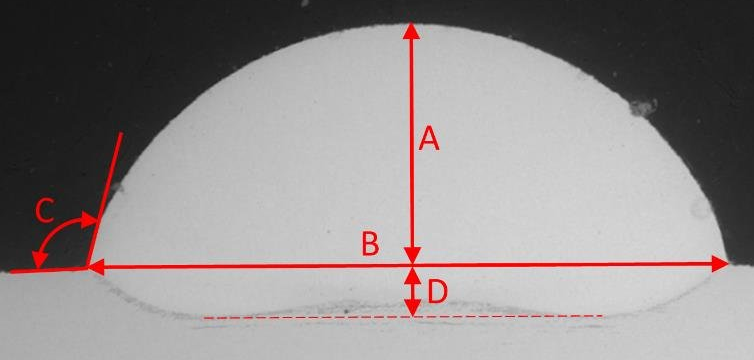
\includegraphics[width=\linewidth]{images/bead_geometry.png}
    \caption{Bead geometry \cite{Dinovitzer_Chen_Laliberte_Huang_Frei_2019}}
    \label{fig:bead_geometry}
\end{figure}

\textbf{Orange box}: Minimum weld quality for overlapping beads.
The bead wall angle, shown as angle $c$ in \autoref{fig:bead_geometry}, should be above 90 $\deg$ for overlapping beads to mix well with each other. All previous beads were quite "steep" ($c \approx 90 \deg$), and in order to get the beads to spread better, higher energy inputs are required. These next tests all used travel speed ramps with fixed feed rates.

Beads 6-8 used 8.5 m/min feed rate and 0.5-0.2 m/min travel rate with varying arc length corrections to try and create higher voltages, although an overprinting error ocurred with bead 8. In an attempt to increase spreading even further, beads 9-10 used 14.5 m/min feed rate and tested the 0.4-1.3 m/min travel speed range, finding 0.8 to be an acceptable condition for overlapping beads.

\textbf{Red box}: Process stability of overlapping beads.
In the red box, this condition was tested with small variations to the initial weld conditions due to the apparent necking ocurring at the start of the bead. SFI time was increased from 0.1 seconds to 1 second to stabilize material deposition, and the initial current was increased to 125\% of the main current.
This did indeed improve the necking somewhat, but induced too much deposition at the weld start. The bead width of the stable overlap condition (0.8 m/min travel speed, 14.5 m/min feed rate) was 5.5 mm.

\textbf{Blue box}: Minimum weld quality of overlapping beads.
The resulting overlap condition from the previous tests was tested with 3-bead overlap with 60\% of the bead width separation, and 5-bead overlap with 70\% separation. The 3-bead overlap showed too much accumulation of material between beads, which is why the distance was slightly increased, resulting in a relatively smooth surface for pieces requiring wider layers.

\textbf{Purple box}: Process stability over many single-bead layers. The three beads shown here are attempts at building walls, all with an average layer height of 2 mm. All three attempts resulted in the same deposition inconsistencies and significant loss of process stability.
For all walls, an interpass temperature of 50$\deg$ was used to ensure that no defects due to overheating might occur. These thermal measurements were sometimes not indicative of the temperature at the topmost layer (due to thermocouple placement or MaxQ thermal camera calibration issues).
The first wall got there after 3 layers, the second after 6, and the heat input was lowered by around 30\% by reuducing the feed rate from 8.5 m/min to 7.3. This allowed the third wall to stay stable up to 10 layers, but the deposition inconsistencies were still present.

Several possibilities for the defects were considered: the arc length may have been too large and not constant enough, allowing the arc to wander and the melt pool to deposit inconsistently. Weld cavities in previous layers would thus be amplified in subsequent layers, and this would be the reason for regularly occuring defects after a set number of layers. The process stability would also be aggravated by a higher heat input.

A final wall was printed on a separate baseplate with a lower heat input at 5.5 m/min feed rate as opposed to 7.3. Defects still ocurred after around 10 layers, as shown in \autoref{fig:big_wall_1}.

\begin{minipage}{\linewidth}
    \centering
    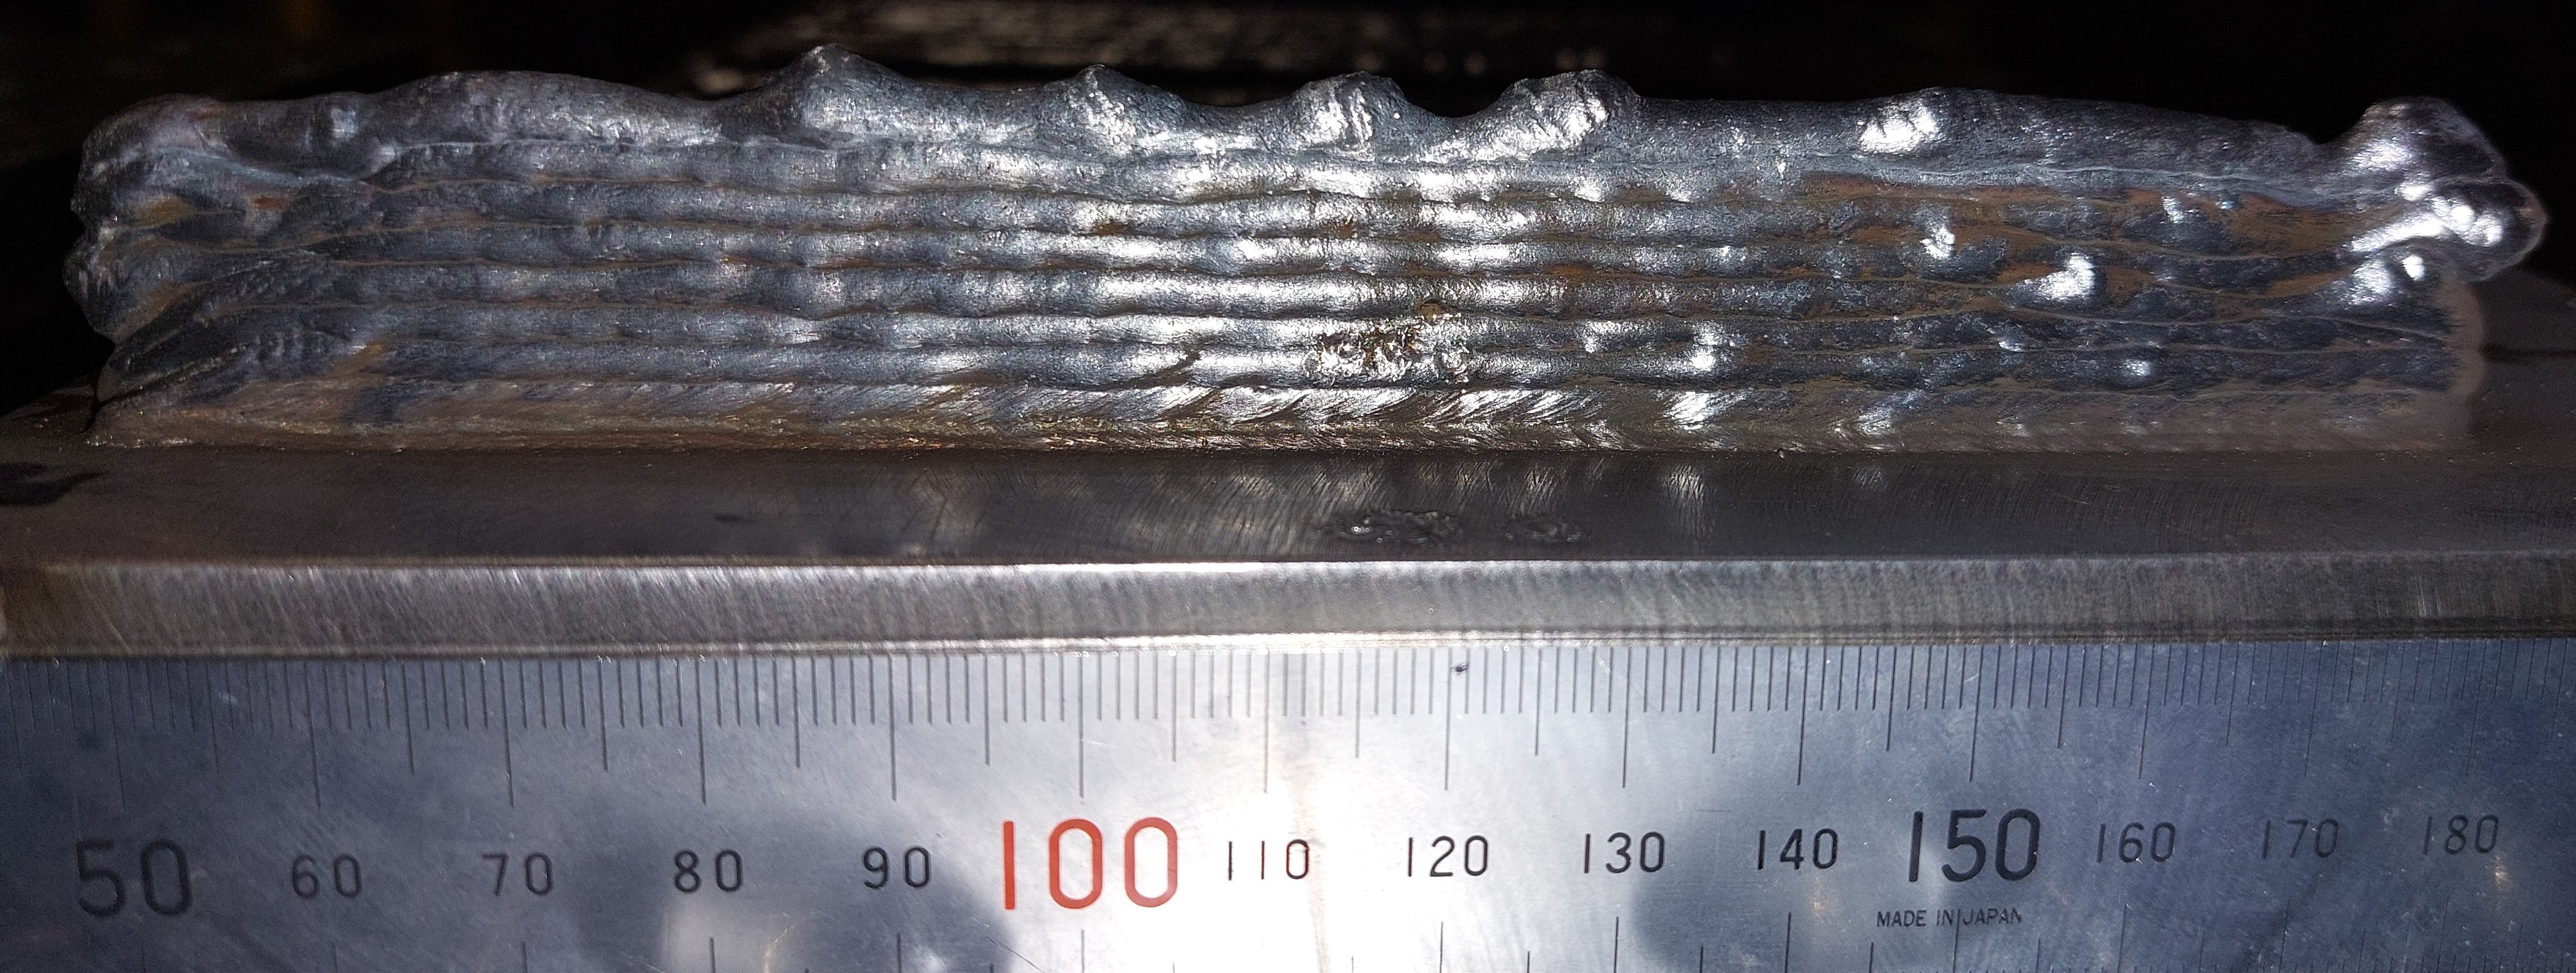
\includegraphics[width=\linewidth]{images/big_wall_1.jpg}
    \captionof{figure}{Final wall test before grinding}
    \label{fig:big_wall_1}
\end{minipage}

This faulty layer was ground to a smooth surface, and an arc length correction of -0.3 was applied, meaning the arc length was reduced by 30\%. This increases the force of the arc on the melt pool by narrowing the arc, and allows for more penetration and re-melting of previous layers to fill in any defects. The resulting wall is shown in \autoref{fig:big_wall_2}, and clearly this change stabilized the process sufficiently to yield relatively smooth layers even after 20 layers.

\begin{minipage}{\linewidth}
    \centering
    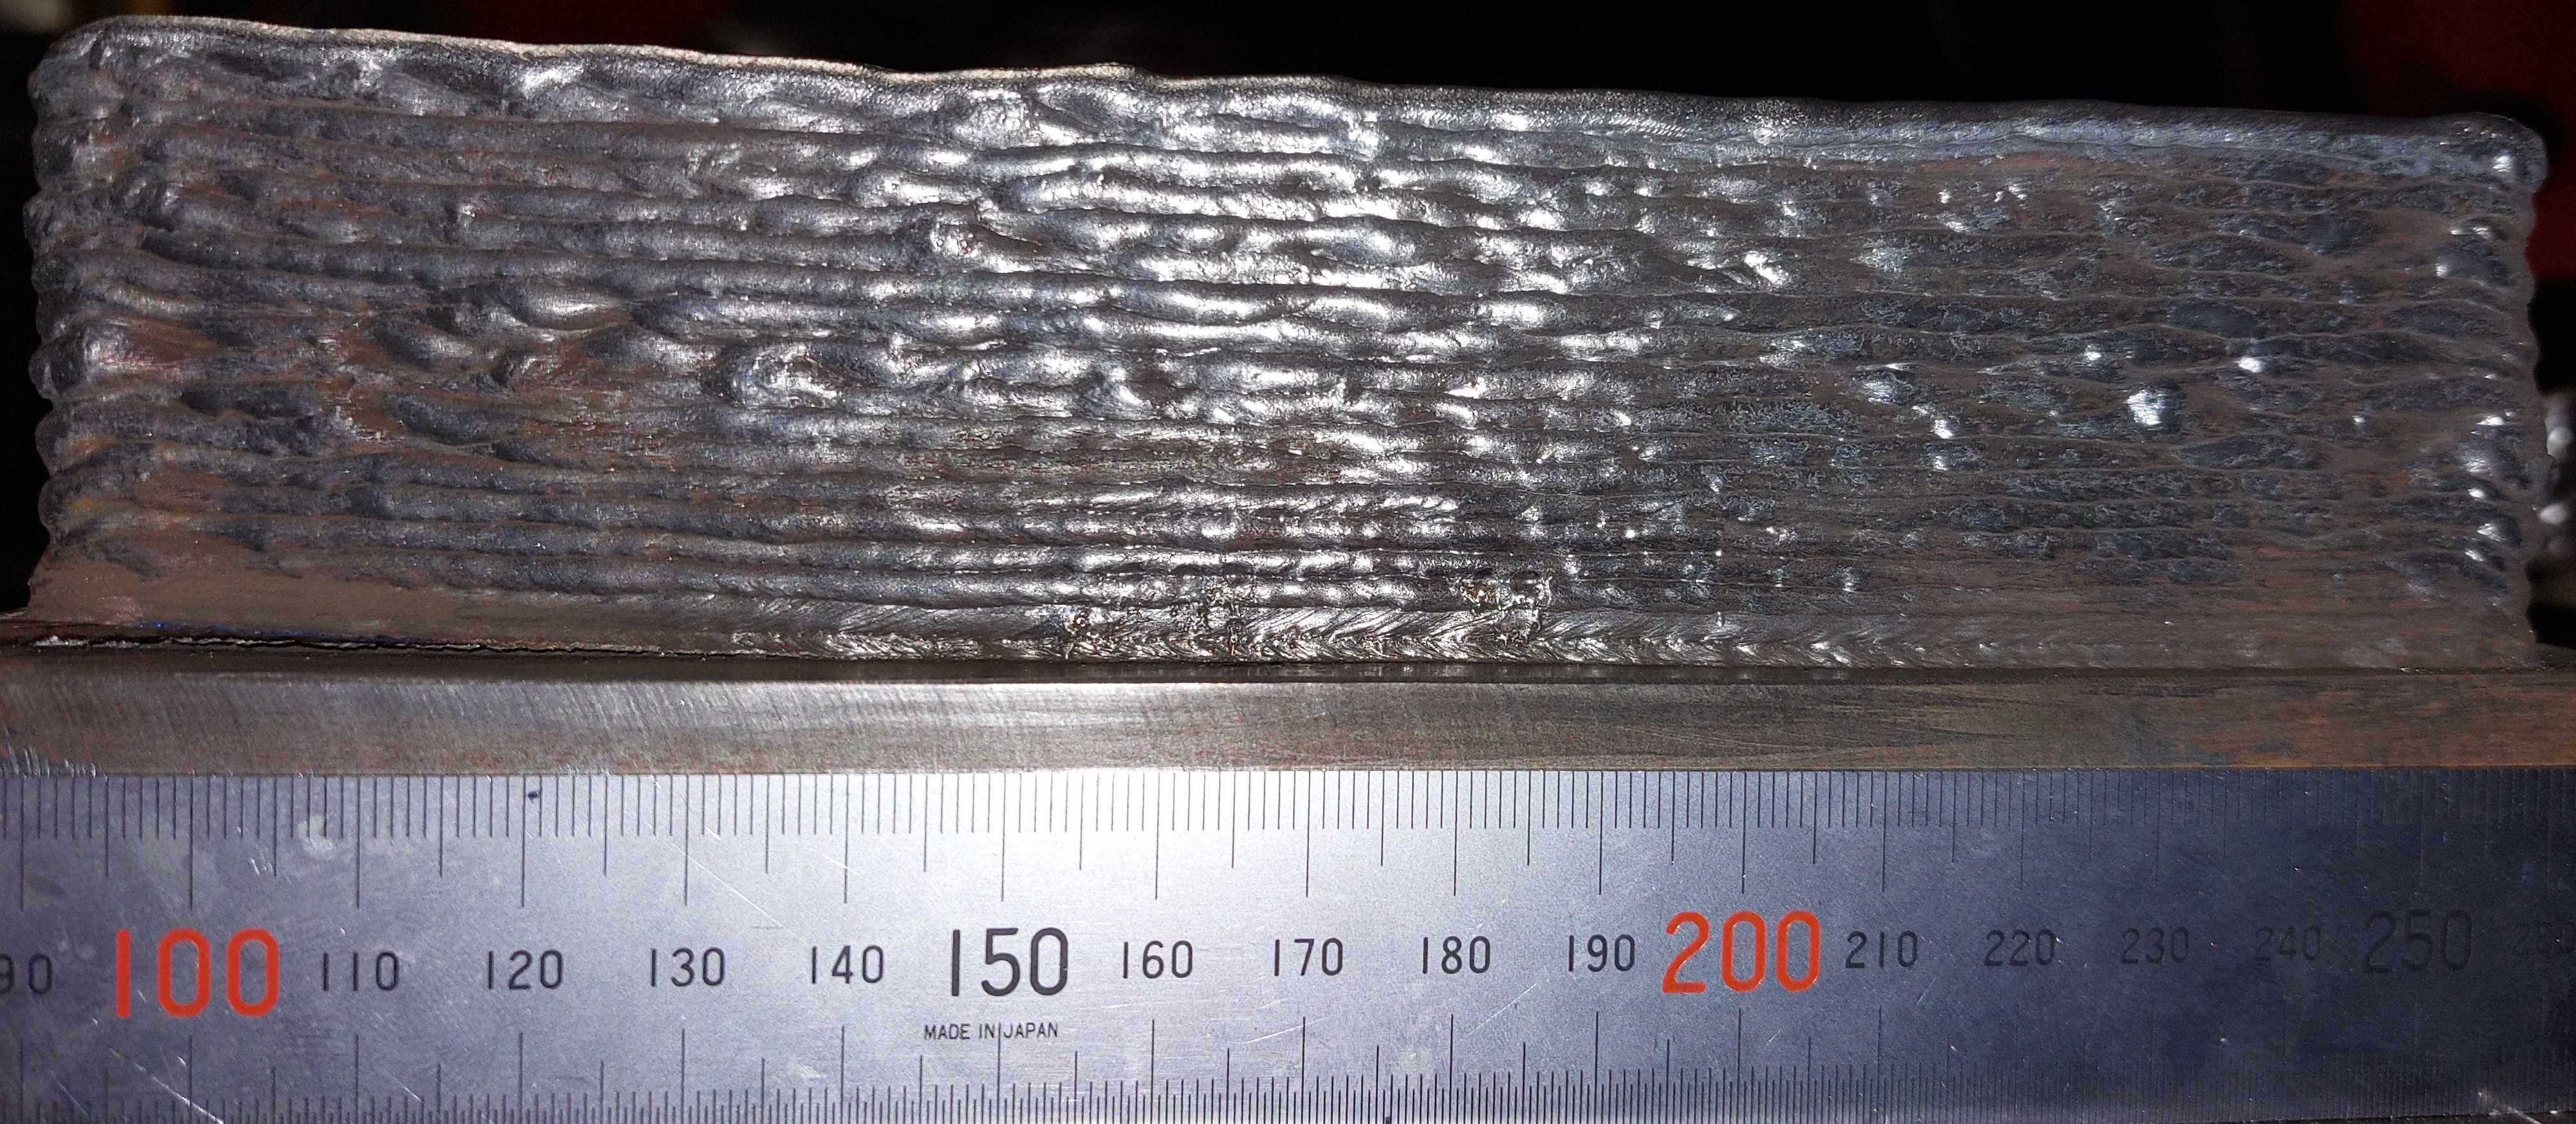
\includegraphics[width=\linewidth]{images/big_wall_2.jpg}
    \captionof{figure}{Final wall test after grinding}
    \label{fig:big_wall_2}
\end{minipage}

Another possible source of inconsistencies was identified after this test: by welding hot, the welding tip can be worn out and its exit hole become larger than desired, as shown in \autoref{fig:tip_hole}. The wire being tested was wound on its spool with residual tension, causing it to come out of the torch at an angle, and this angle can change over time duing welding, deflecting the arc from the intended bead path, causing the same kind of arc and melt pool wandering described earlier.

\begin{minipage}{\linewidth}
    \centering
    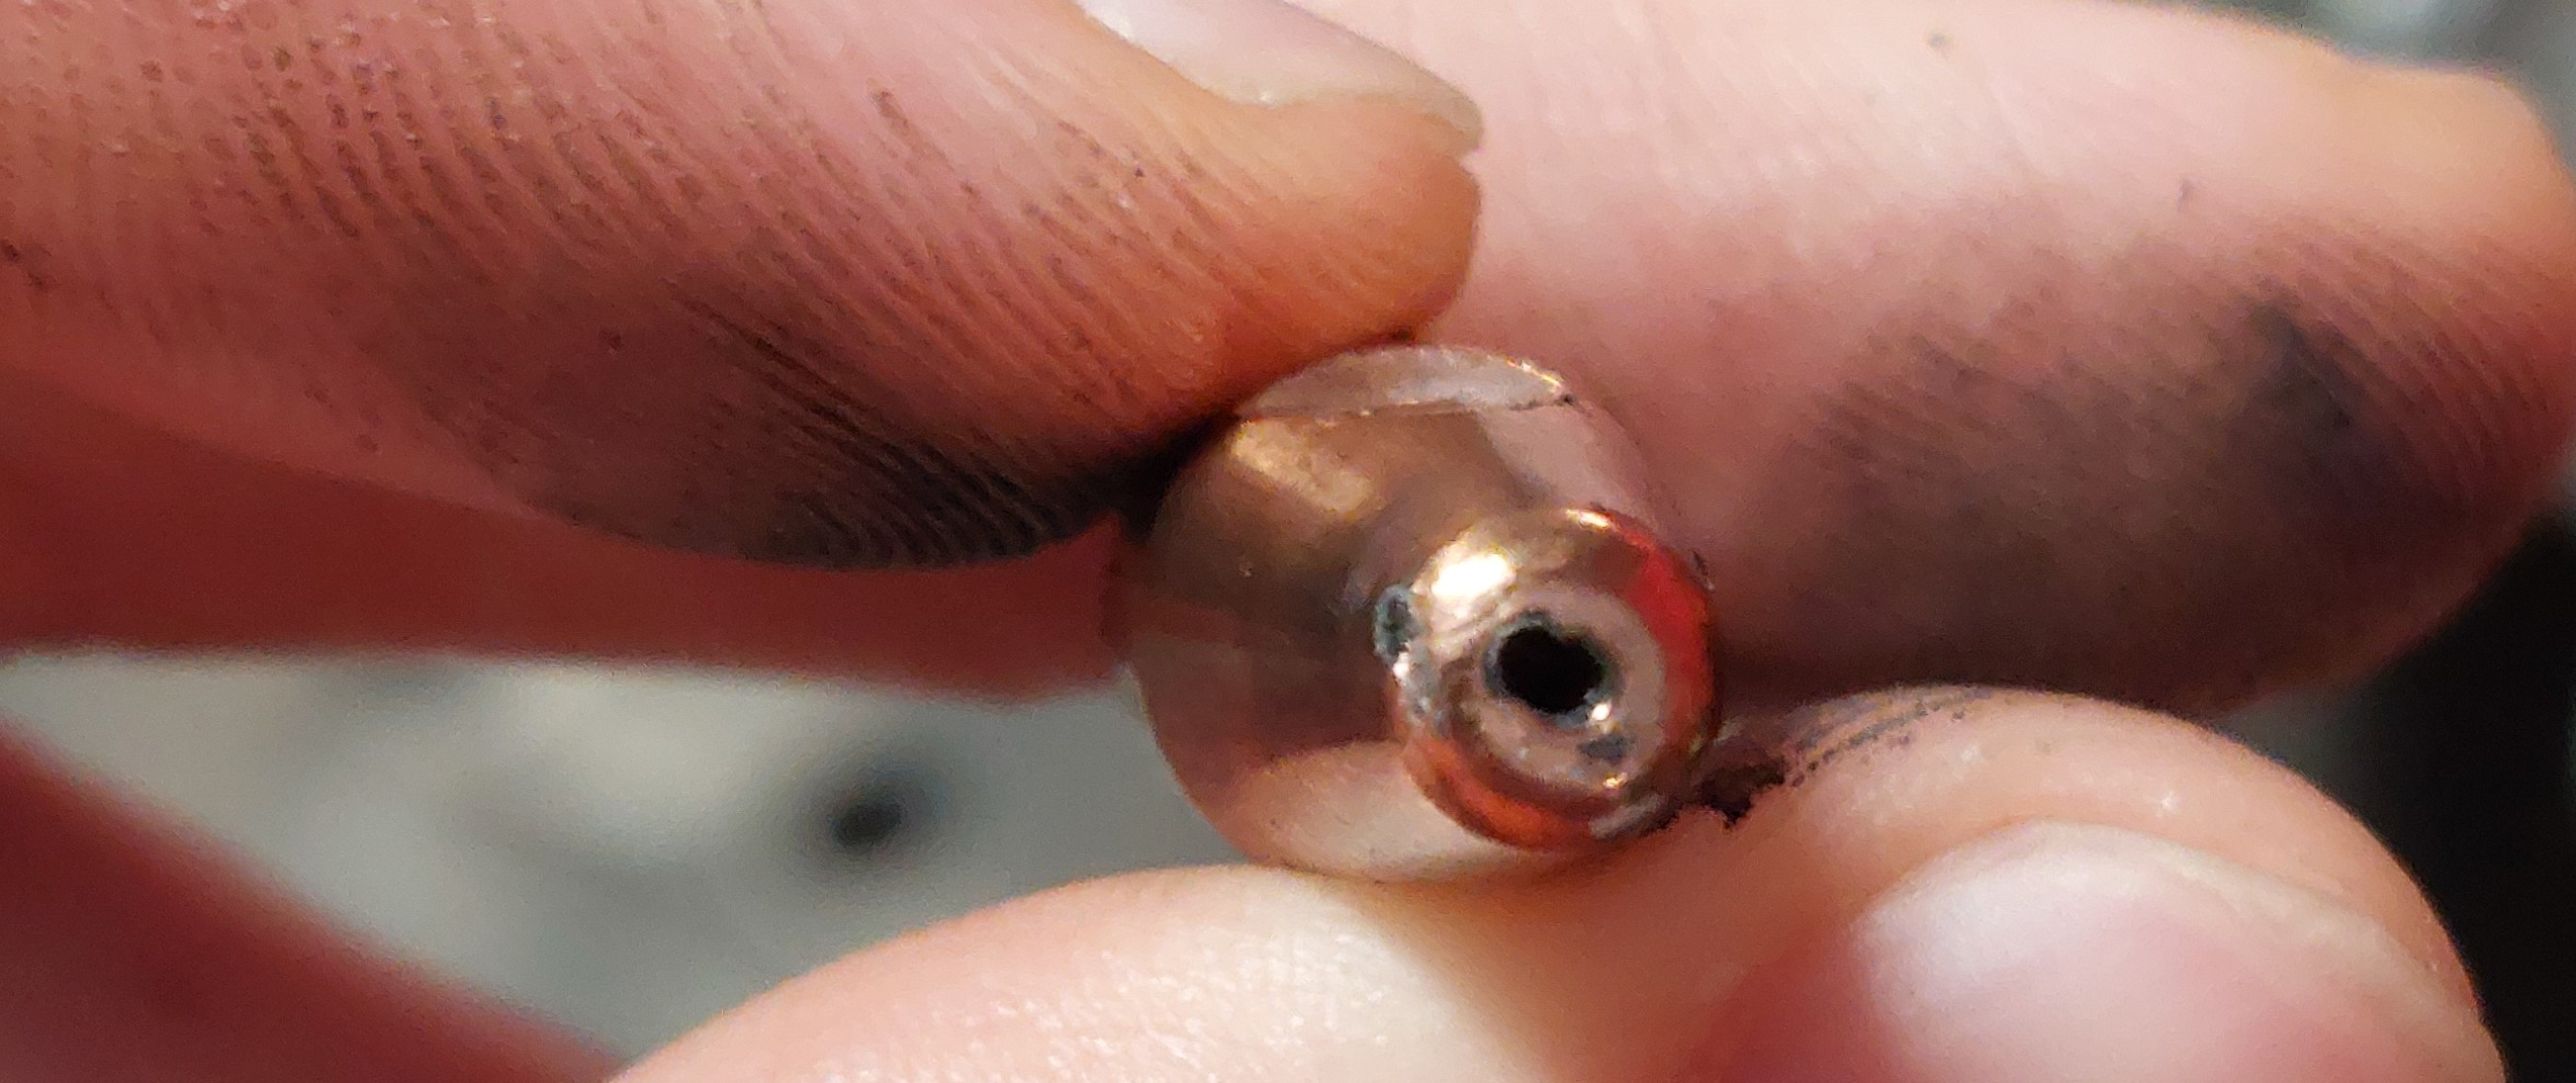
\includegraphics[width=\linewidth]{images/tip_hole.jpg}
    \captionof{figure}{Tip hole wearing out}
    \label{fig:tip_hole}
\end{minipage}

After the establishment of successful single-bead layers, the next milestone was the minimum print quality for a full-scale part. The chosen geometry was a simple set of concentric rings, and the initial tests were conducted on a single ring.
This involved manually rotating the layer toolpaths around the center axis to randomize the start/stop points of the beads to prevent defects from accumulating in the same place, as well as alternating the direction of welding. The resulting ring is shown in \autoref{fig:ring_1}.

\begin{minipage}{\linewidth}
    \centering
    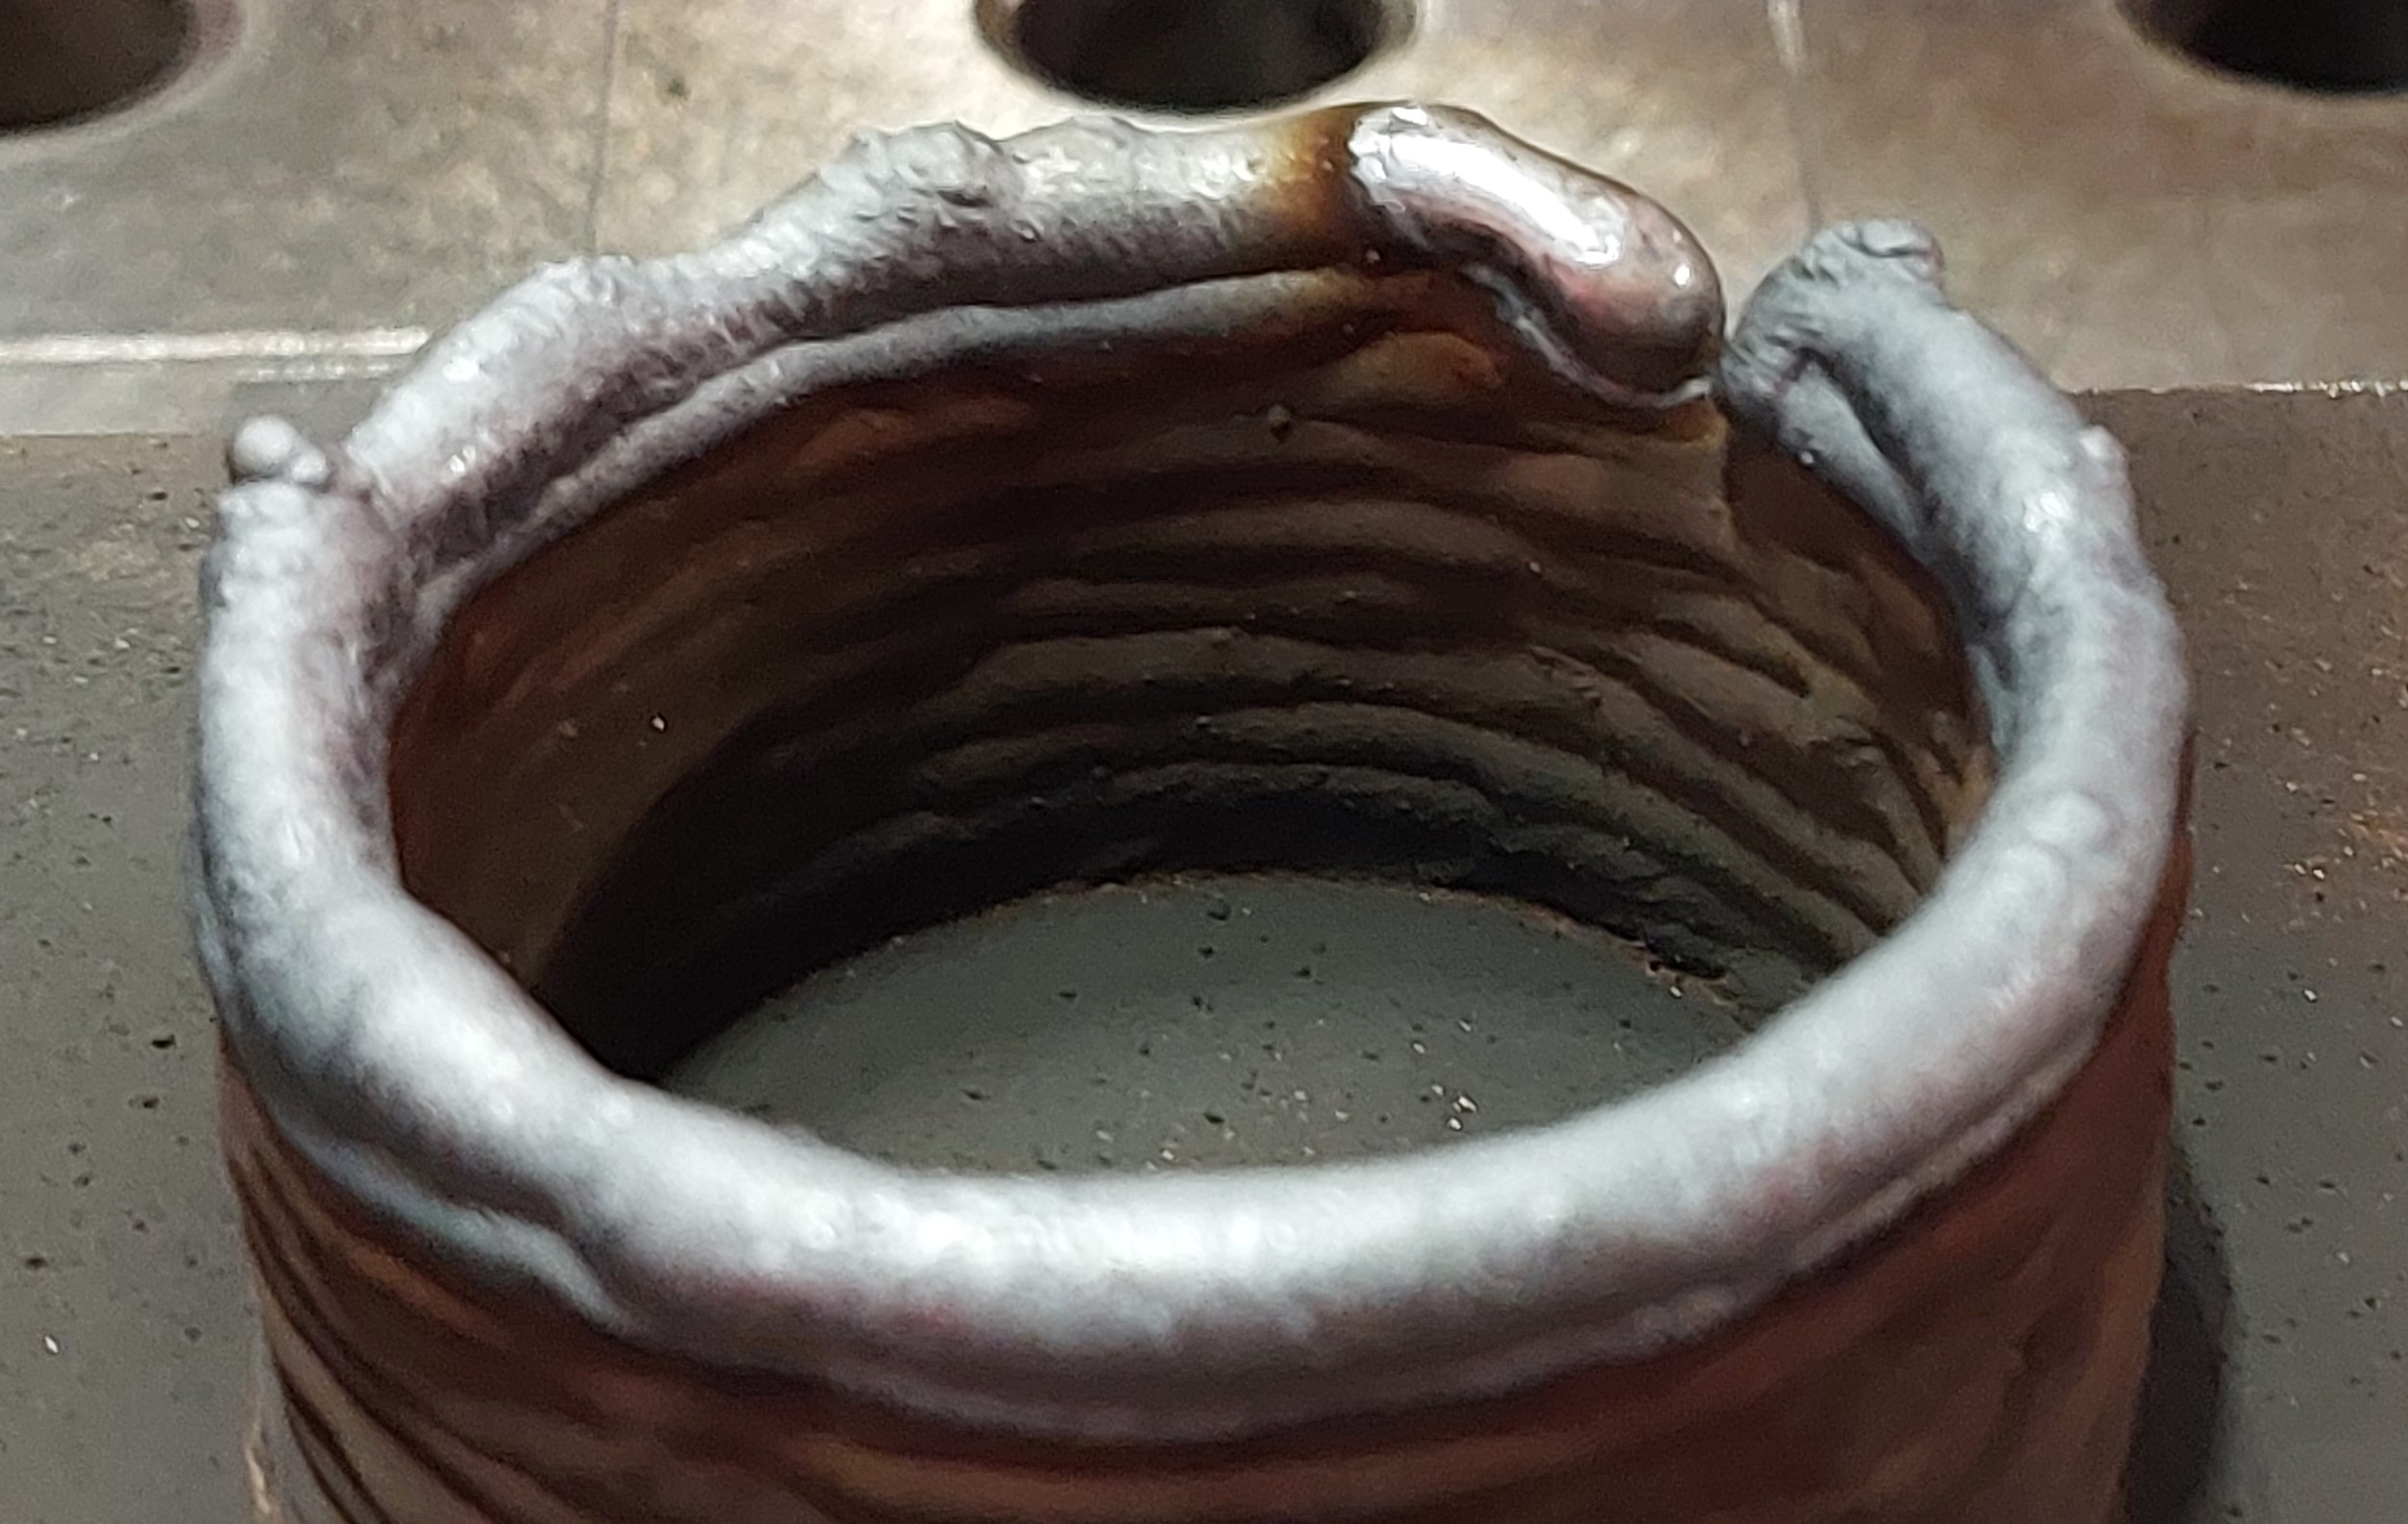
\includegraphics[width=\linewidth]{images/ring_1.jpg}
    \captionof{figure}{First ring test with defect}
    \label{fig:ring_1}
\end{minipage}

The rather large defect was caused by a previous layer containing a large valley, and the arc being unable to close it, as shown in \autoref{fig:ring_defect}.

\begin{minipage}{\linewidth}
    \centering
    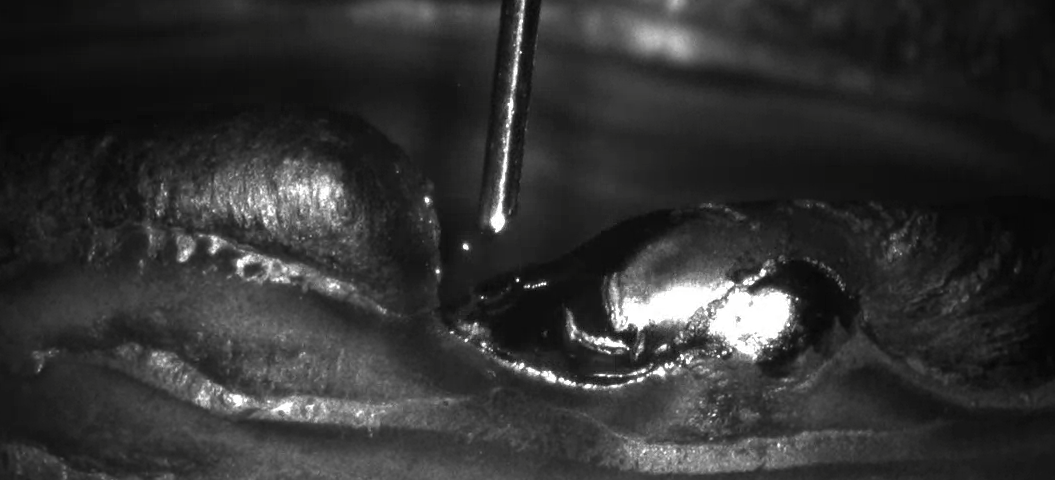
\includegraphics[width=\linewidth]{images/ring_defect.PNG}
    \captionof{figure}{Moment of inability to close gap in first ring test}
    \label{fig:ring_defect}
\end{minipage}

Welding was filmed using the previously mentioned Cavitar camera, and analysing the solidification of the melt pool in real-time showed that the source of the defects was not thermal, but rather possibly due to the effects of the oxygen in the atmosphere pulling the elements in the melt pool outwards, causing "bubbling" outgrowths as shown in \autoref{fig:bubble_defect}.

\begin{minipage}{\linewidth}
    \centering
    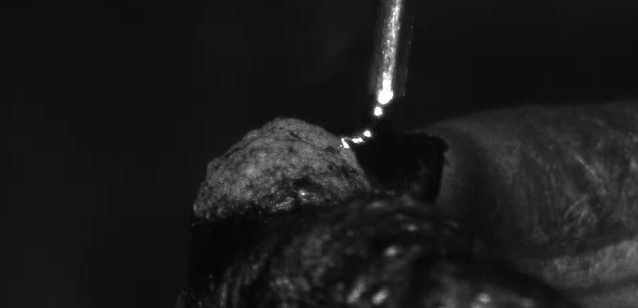
\includegraphics[width=\linewidth]{images/bubble_defect.PNG}
    \captionof{figure}{Bubble outgrowths during welding}
    \label{fig:bubble_defect}
\end{minipage}

This effect would be pronounced in higher layers due to less of the base plate impeding the shielding gas' flow and keeping it in contact with the melt pool for longer, which might have explained why defects consistently ocurred once a certain wall height was reached.

In order to prolong the contact time of the shielding gas with the weld pool, the travel speed was reduced from 0.3 to 0.25 m/min. The interpass temperature was also increased from 50$\deg$ to 80$\deg$ to reduce cooling times and increase the likelihood of layer remelting. A second ring was printed with these conditions, as shown in \autoref{fig:ring_2}.
This ring was the first wall to be printed without any significant defects occurring - most likely due to the mitigation of the oxygen effects by the slower travel speed, and the increased heat input allowing for more re-melting of previous layers to fill in any defects. This second point is important, since defects cannot be prevented, but they can be corrected through remelting.

\begin{minipage}{\linewidth}
    \centering
    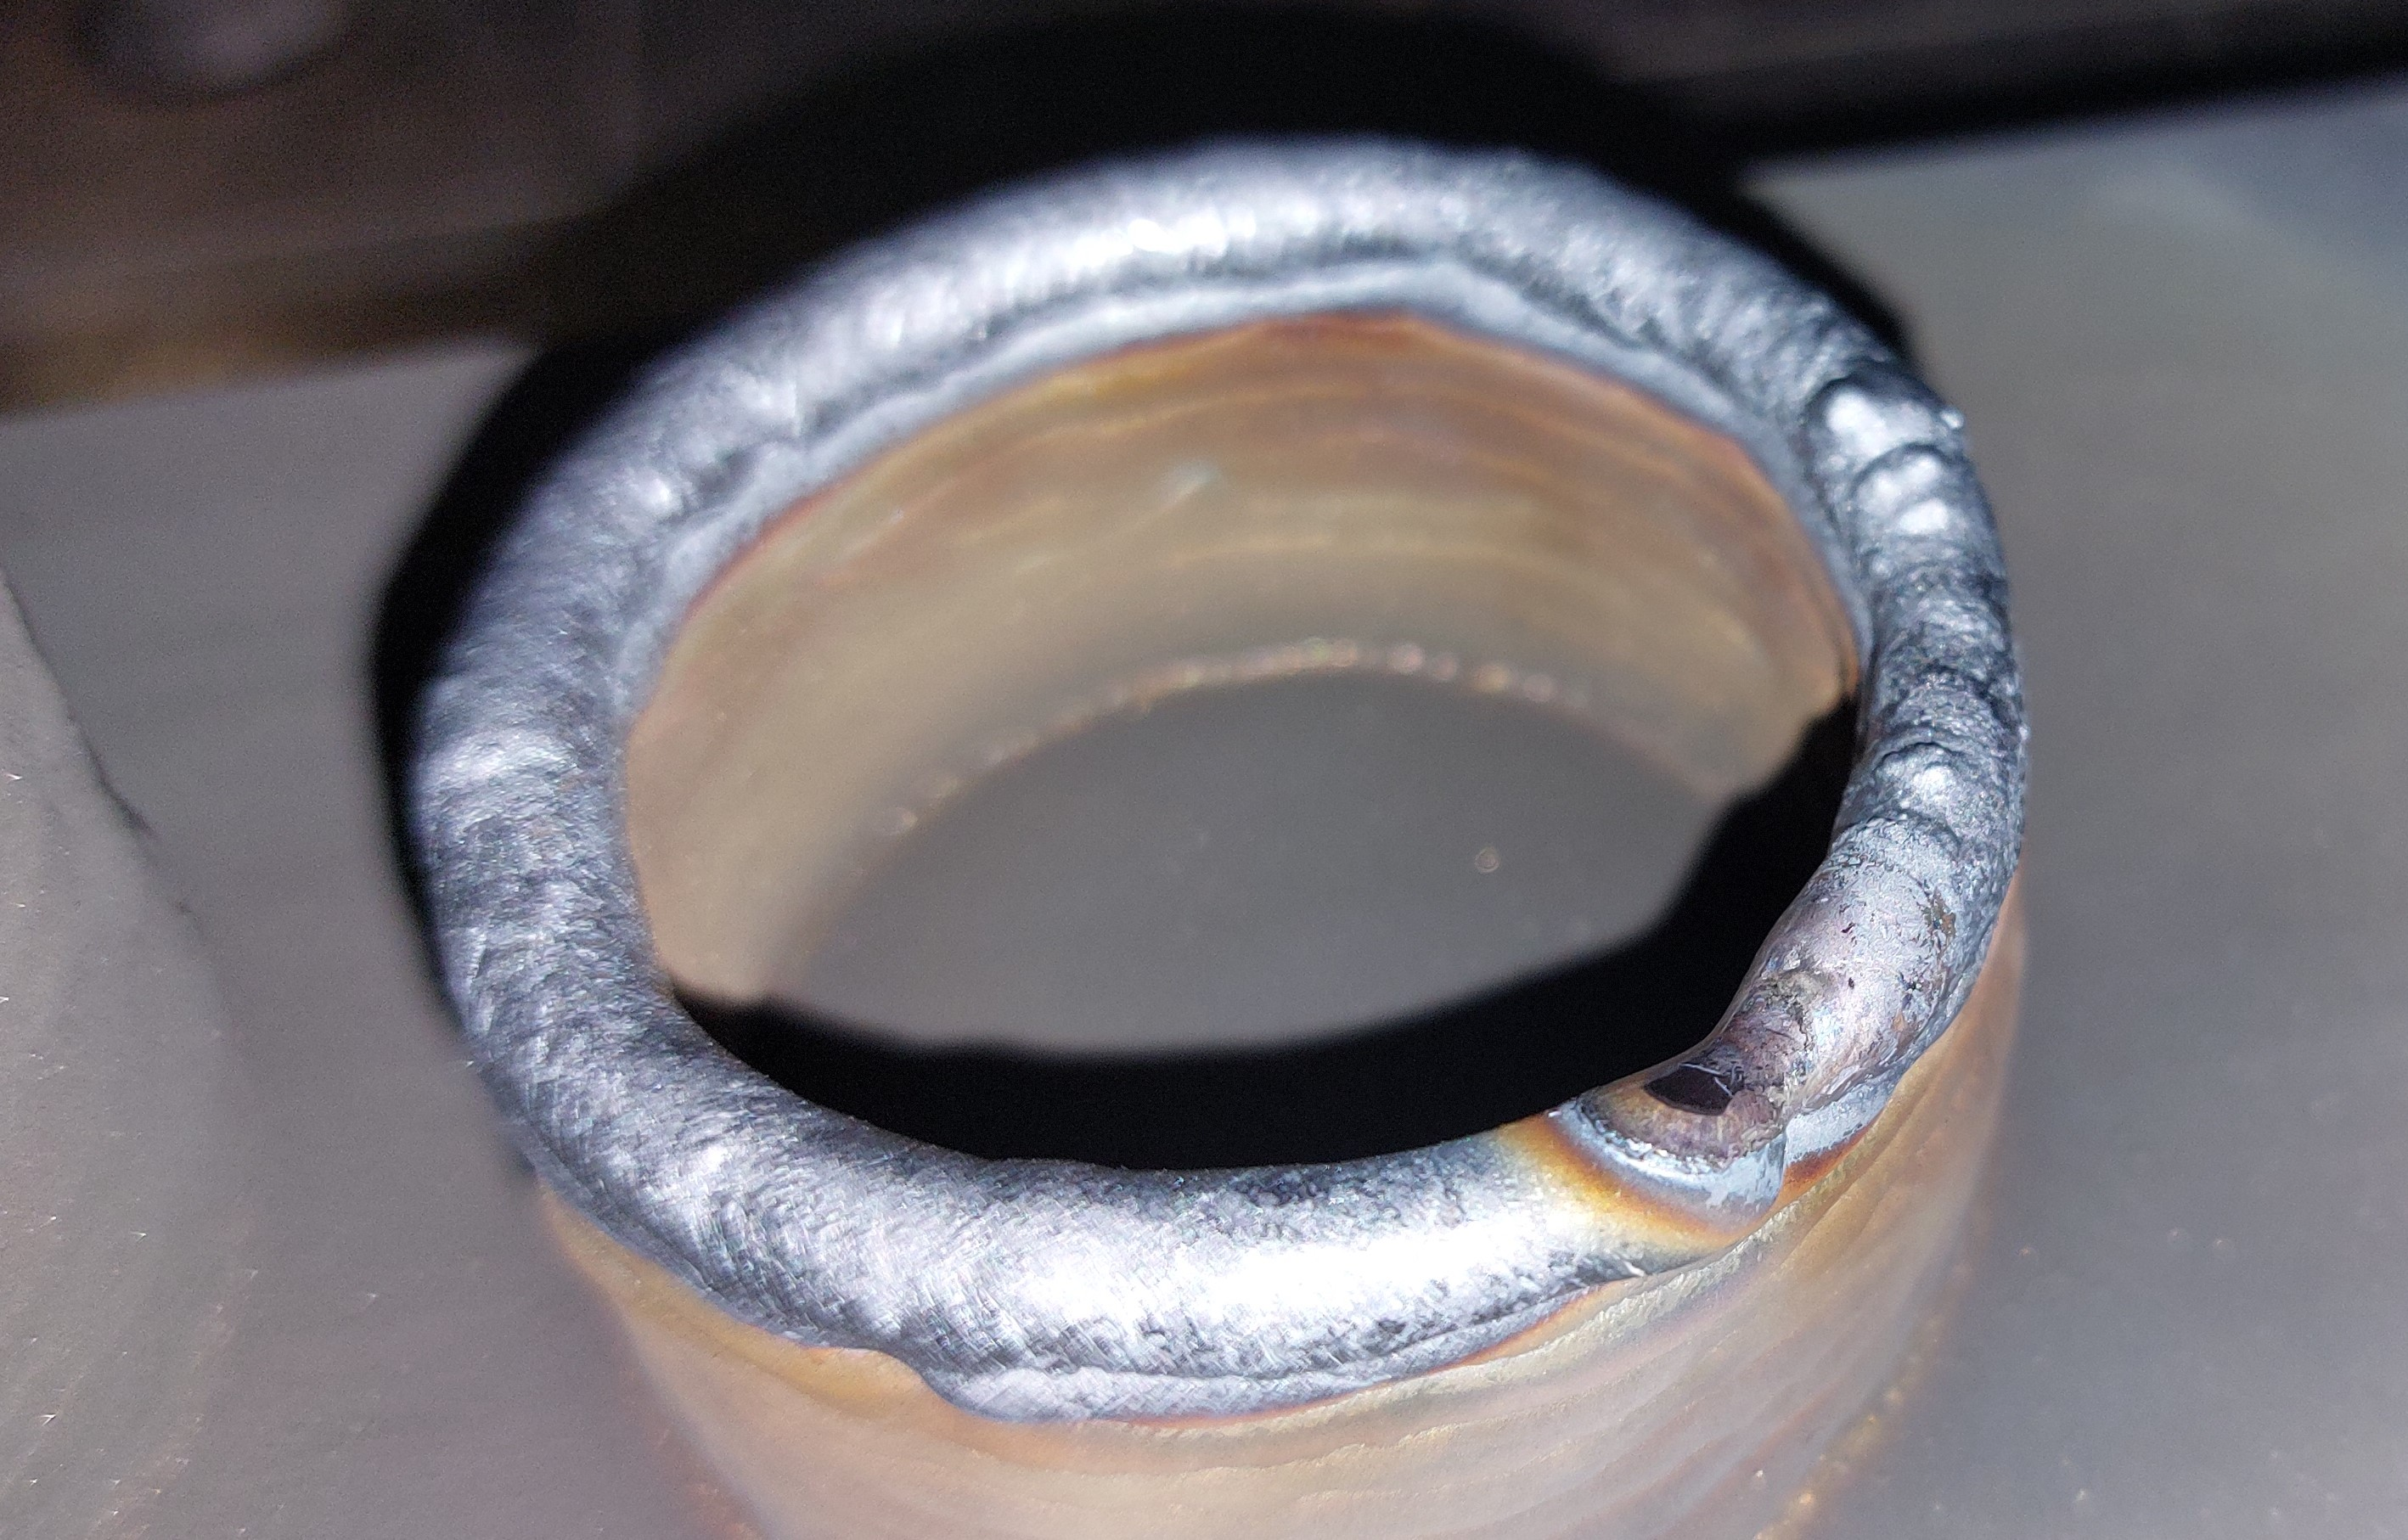
\includegraphics[width=\linewidth]{images/ring_2.jpg}
    \captionof{figure}{Second ring test with no defects}
    \label{fig:ring_2}
\end{minipage}

With this relatively stable condition achieved, this ring was used for sample collection for microscopy and magnetic testing. The tests moved on to printing full geometries consisting of two concentric rings on much smaller baseplates, which are commonly used in production scenarios. This introduced a new issue of thermal loading and excessively long cooling times due to the comparatively small thermal reservoir a smaller baseplate offers.

\begin{minipage}{\linewidth}
    \centering
    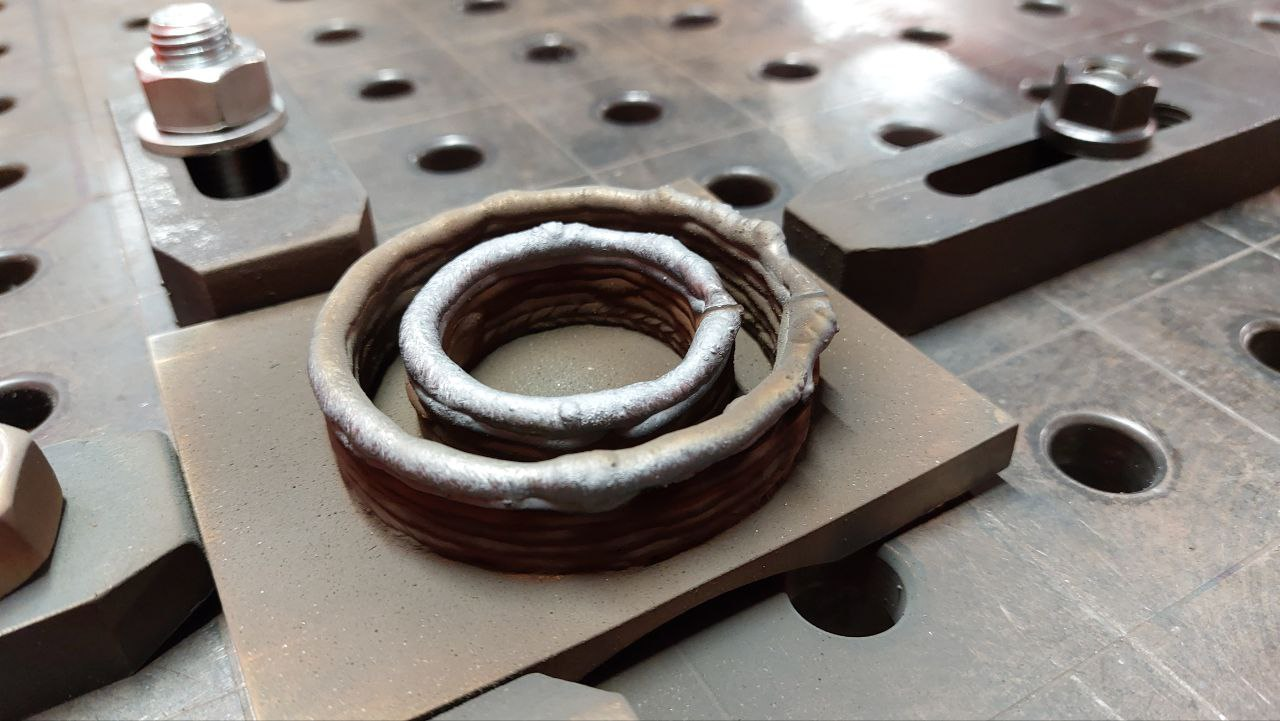
\includegraphics[width=\linewidth]{images/photo_2023-11-14_15-40-54.jpg}
    \captionof{figure}{First full geometry print in progress}
    \label{fig:half_ring_bending}
\end{minipage}

As shown in \autoref{fig:half_ring_bending}, the corners of the small baseplate are lifted due to repeated heating, and we begin to see the development of so-called "humps" after a few layers. The first few layers in this print were fully smooth and stable. We considered that the bending of the plate may have introduced wire tip positioning errors and thus induced instabilities, so the MaxQ geometrical scanning system was configured for the next print. This system projects the planned toolpath on the existing geometry and adjusts the vertical distance to the part accordingly to keep a stable Contact Tube to Work Piece (CTWD) distance. All subsequent prints made use of this distance correction through 3D scanning. 

\begin{minipage}{\linewidth}
    \centering
    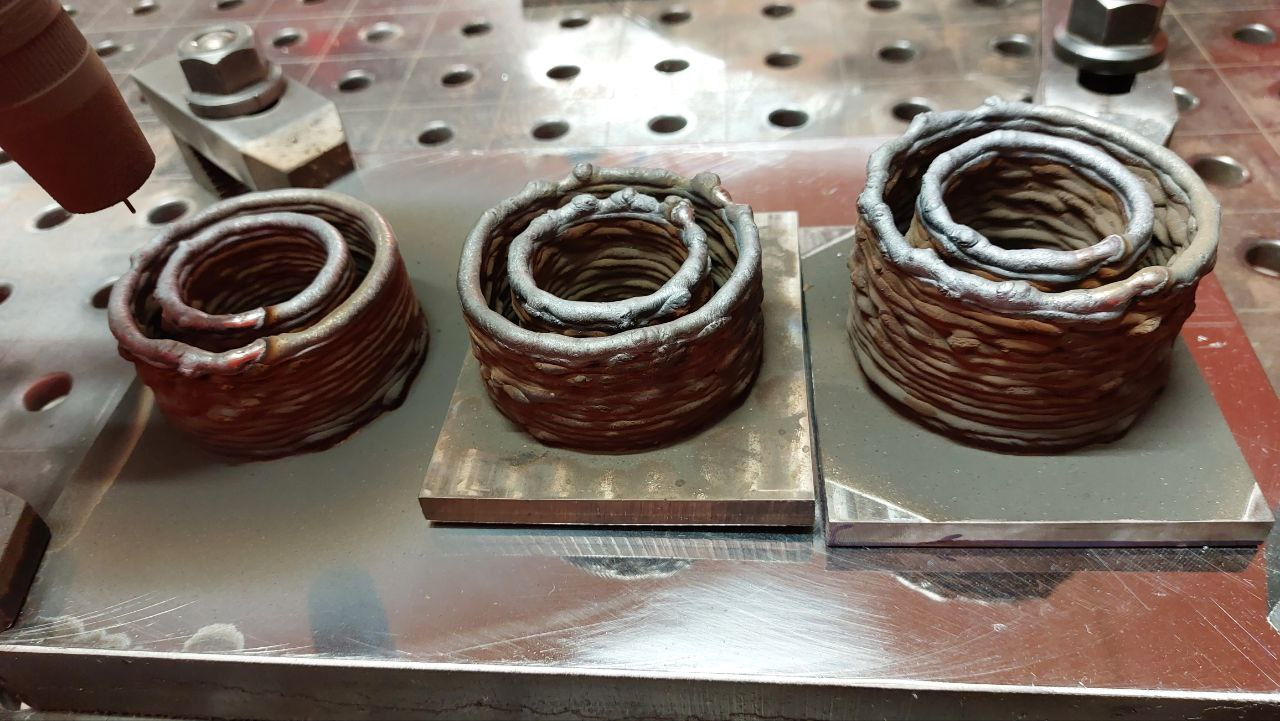
\includegraphics[width=\linewidth]{images/photo_2023-11-14_15-39-49.jpg}
    \captionof{figure}{Three full geometry attempts}
    \label{fig:3_rings}
\end{minipage}

\autoref{fig:3_rings} shows three subsequent tests at printing the full geometry in varying conditions. In the center is the finished piece previously shown in \autoref{fig:half_ring_bending}, which was printed with an interpass temperature of 80 $^o$C, displaying significant defects on its top layer. On the right, the following print can be seen. The shielding gas flow rate, which was previously 22 L/m, was increased to 24 L/m. Because of the baseplate's composition (also Vacoflux 17), wettability issues had been identified elsewhere and mitigated with a heat input increase of 15\%, 10\% and 5\% for the first three layers. This was also done for this print. 3D scanning was used along with clamps on the edges of the baseplate to address bending and thus mitigate positioning issues. The interpass temperature was also set to 120 $^o$C to reduce cooling times, but still with all of these process changes, defects still occurred to a significant degree. The hypothesis arose that this may be due to the melt pool staying hot for too long (due to poor thermal conduction of the thin walls of the part), and being exposed to the atmosphere while still in a liquid state, causing reactions with the oxygen present.

As pictured on the very left, another test was run on a large baseplate. This was done to examine whether the thermal issues were the true cause behind the "hump" defects. The interpass temperature was lowered to 50 $^o$C, and additionally, a leading angle of 10 degrees (i.e. the tip tilted in the direction of travel) was introduced in order to push the melt pool forwards, remelting defective layers, instead of backwards, where the forces might accumulate to further defects. Even with these process parameter changes, the defects continued to occur, although quite often, it was possible to remelt previously defective layers.

It must be said that for all of these "humping" and (as mentioned above) "bubbling" defects, the location of the errors was seemingly random and did not follow any discernible patterns. Previous defects were more often than not successfully corrected by a new layer, which in turn had new defects in a different part of the ring.

% \subsection{Software defects}

% ROS bridge
% Decryption of the Techman
% Post-processor minor errors
% Techman weirdness (not starting, bugging out)
% TCP errors
% MaxQ 3D camera calibration issues

\begin{table*}[ht]
\centering
\caption{VSM Hysteresis Loop Results}
\label{tab:mag_data}
\begin{tabular}{|l|l|l|l|l|l|}
\hline
\textbf{Property/Sample} & \textbf{Wire} & \textbf{Weld} & \textbf{Ar} & \textbf{H} & \textbf{H \%} \\ \hline
\textbf{Coercivity [A/m]}         & 530.78   & 659  & 934  & 362  & -31.87 \\ \hline
\textbf{Remanence [A/m]}          & 34.94    & 32.2 & 25.4 & 18.3 & -47.56 \\ \hline
\textbf{Sat. Magnetization [A/m]} & 1906.847 & 1883 & 1832 & 1821 & -4.46  \\ \hline
\textbf{Max. Permeability [H/m]}  & 5240.246 & 3810 & 3002 & 4009 & -23.49 \\ \hline
\textbf{Hysteresis Area [J/m$^3$]}  & 36.377   & 39.9 & 34.8 & 26.5 & -27.28 \\ \hline
\end{tabular}
\end{table*}



\section{Magnetic Results}

In order to investigate the effects that welding have on the magnetic performance of the material, samples at differing degrees of processing were taken and tested. An unaltered Vacoflux 17 wire was tested, as were a welded sample and two annealed ones.

The magnetic characterization of the samples consisted of a VSM test performed at the TU Delft 3ME laboratory. From the successful ring printed as shown in \autoref{fig:ring_2}, a cross-sectional sample was taken. From the uppermost layer of this cross-section, a 2x2x2 mm sample was cut, since this was the maximum sample volume for the VSM. The rest of the cross-section was split and used for annealing.

The recommended annealing is specified by the manufacturer in Vacoflux 17's data sheet as 850 C for 10 hours in a hydrogen atmosphere, followed by a cooling rate of 100-200 C/h. Hydrogen is relatively expensive and can cause leaks, so a first annealing with pure Argon was attempted to verify whether the process could be performed by a cheaper and more stable gas. The second annealing was performed as intended by the manufacturer.

Table XXX shows the relevant and testable parameters for the five conditions: as tested by the manufacturer, and the four samples taken by the author.

\begin{table*}[t]
    \centering
    \caption{Magnetic performance across samples}
    % \label{tab:mag_data}
    \begin{tabular}{llllll}
    Property/Sample         & Man.    & Wire  & Weld & Ar    & H \\
    Coercivity [A/m]        & 140     & 531   & 659  & 934   & - \\
    Remanence [A/m]         & -       & 34.94 & 32.2 & 25.35 & - \\
    Sat. Mag. [A/m]         & 1.803e6 & 1907  & 1883 & 1832  & - \\
    Max. Perm. [H/m]        & 3200    & 5240  & 3810 & 3002  & - \\
    Hysteresis Area [$J/m^3$] & -     & 36.4  & 39.9 & 34.8  & - \\
    \end{tabular}
\end{table*}



\section{Conclusions/Recommendations}

There are three main points to be made given the results of this investigation so far:

\begin{itemize}
    \item Vacoflux-17 can be printed with a relatively high quality and accuracy using MIG WAAM under certain conditions.
    \item There are "bubbling" and "humping" defects which occur consistently in single-bead walls after enough layers have been built up. These defects are not well understood, and persist even after mitigation attempts using 6-7 different strategies failed. It is surmised that these defects can be solved through process parameter optimization and yet unexplored modifications.
    \item Welding worsens the material's magnetic performance, but annealing in a H$_2$ atmosphere for 10 hours at 850 $^o$C corrects this loss, and even improves on the wire's baseline performance. More tests, like a permeameter, are needed to more fully characterize the material's magnetic performance in different regimes, like AC loading.
    \item The microstructure and compositional tests have not yet been completed, but will be included in this point when they soon are.
\end{itemize}

\section{Recommendations}



\bibliographystyle{plain} % We choose the "plain" reference style
\bibliography{refs} % Entries are in the refs.bib file

\end{multicols}
\end{document}
